\documentclass[twocolumn,10pt]{article}

\usepackage[a4paper,hmargin=1.5cm,vmargin=2cm]{geometry}
\setlength{\columnsep}{0.7cm}
%\usepackage{microtype} % nice typesetting  % doesn't work for me :-( -S
\usepackage{amsmath}
\usepackage{graphicx}
\usepackage{caption}
\usepackage{balance}
\usepackage{palatino}
\usepackage[varqu]{inconsolata}

\usepackage[utf8]{inputenc}
\usepackage{natbib}
\bibliographystyle{simon}
\setlength{\bibsep}{0.3ex plus 0.2ex}
%\setcitestyle{aysep={}} 
\usepackage[dvipsnames]{xcolor}
\usepackage[compact]{titlesec}
\usepackage[hypertexnames=false]{hyperref}
\hypersetup{
    colorlinks,
    linkcolor={blue!50!black},
    citecolor={blue!50!black},
    urlcolor={blue!50!black}
}
\urlstyle{same} % no tt font for URLs
\renewcommand{\topfraction}{0.9}
\renewcommand{\dbltopfraction}{0.9}
\renewcommand{\textfraction}{0.1}
\clubpenalty=1000
\widowpenalty=1000
\displaywidowpenalty=1000


\newcommand\blfootnote[1]{%
    \begingroup
    \renewcommand\thefootnote{}\footnote{#1}%
    \addtocounter{footnote}{-1}%
    \endgroup
}

\newcommand{\todo}[1]{[\textcolor{orange}{#1}]}

\begin{document}

\twocolumn[{%
\centering
\textbf{\Large Analyzing single-cell bisulfite sequencing data with \texttt{scbs}}\\[1.5ex]

Lukas P.~M. Kremer\textsuperscript{1,2,*}, Martina Braun\textsuperscript{2}, Leonie Küchenhoff\textsuperscript{1,2}, Santiago Cerrizuela\textsuperscript{2},\\Ana Martin-Villalba\textsuperscript{2}, Simon Anders\textsuperscript{1,*}\\[1ex]
{\footnotesize \textsuperscript{1} BioQuant Centre, University of Heidelberg, Heidelberg, Germany\\[-.5ex] 
\textsuperscript{2} Molecular Neurobiology Dept., German Cancer Research Center (DKFZ), Heidelberg, Germany}
\vspace{1.5ex}

April 2023
\vspace{5.5ex}

\begin{minipage}{0.7\textwidth}
\small \setlength{\parindent}{1em}
\noindent \textit{Abstract} -- Single-cell bisulfite sequencing (scBS) is a technique that enables the assessment of DNA methylation at single-base pair and single-cell resolution. The analysis of the large datasets obtained from scBS requires preprocessing to reduce data size, improve signal-to-noise ratio, and provide interpretability. Typically, this is achieved by dividing the genome into large tiles and averaging the methylation signals within each tile.

Here, we demonstrate that this coarse-graining approach can lead to signal dilution, and propose improved strategies to identify more informative regions for methylation quantification, and a more accurate quantitation method than simple averaging. Our approach enables better discrimination of cell types and reduces the need for large numbers of cells. We also present an approach to detect differentially methylated regions (DMRs) between groups of cells, and demonstrate its ability to identify biologically meaningful regions that are associated with genes involved in the core functions of specific cell types.

To facilitate the analysis of scBS data, we have developed a software tool called ``\texttt{scbs}'' that implements these methods and provides additional functionality.

%In summary, our work provides a more robust and accurate approach to analyze scBS data, which has the potential to enhance our understanding of DNA methylation dynamics in single cells and improve the identification of epigenetic changes associated with different cell states or diseases.
\end{minipage}
\vspace{6.5ex}
}]
\setcounter{secnumdepth}{0} 

\section{Introduction}

Sequencing-based assays with single-cell resolution have offered new means to understand the differences between the cells making up a sample.
Single-cell RNA sequencing (scRNA-seq) techniques have matured at great pace in recent years, with well developed analysis methodology, and methods to study epigenetics at single-cell resolution are rapidly catching up.


Here, we discuss bisulfite sequencing, a method to study DNA methylation.
In brief, DNA is treated with bisulfite, which converts unmethylated cytosines to uracils which are read as thymine in subsequent PCR, while methylated cytosines are protected from conversion.
After sequencing, these conversions allow to determine the methylation status of all cytosines covered by reads \citep{Frommer_1992}.
Bisulfite sequencing can also be performed at single-cell resolution \citep{Smallwood_2014} and even in parallel with scRNA-seq \citep{scMTseq,Clark2018}.

In the present paper, we discuss strategies to analyze single-cell bisulfite-sequencing (scBS) data. We suggest improvements to current approaches, and demonstrate their value in benchmarks, using two real-world datasets. Furthermore, we discuss how to perform comparative analyses. Finally, we present ``scbs'', a comprehensive software toolkit to perform scBS data analysis, using the described methods. 
\blfootnote{\hspace{-.5cm}\raggedright\textsuperscript{*} e-mail:  \texttt{l.kremer@dkfz-heidelberg.de} and\\ \hspace{1cm}\texttt{simon.anders@bioquant.uni-heidelberg.de}}


%\phantomsection  % idk why we need this to silence hyperref's warning
\subsection{Standard approach}

\begin{figure*}[t]
    \begin{center}
        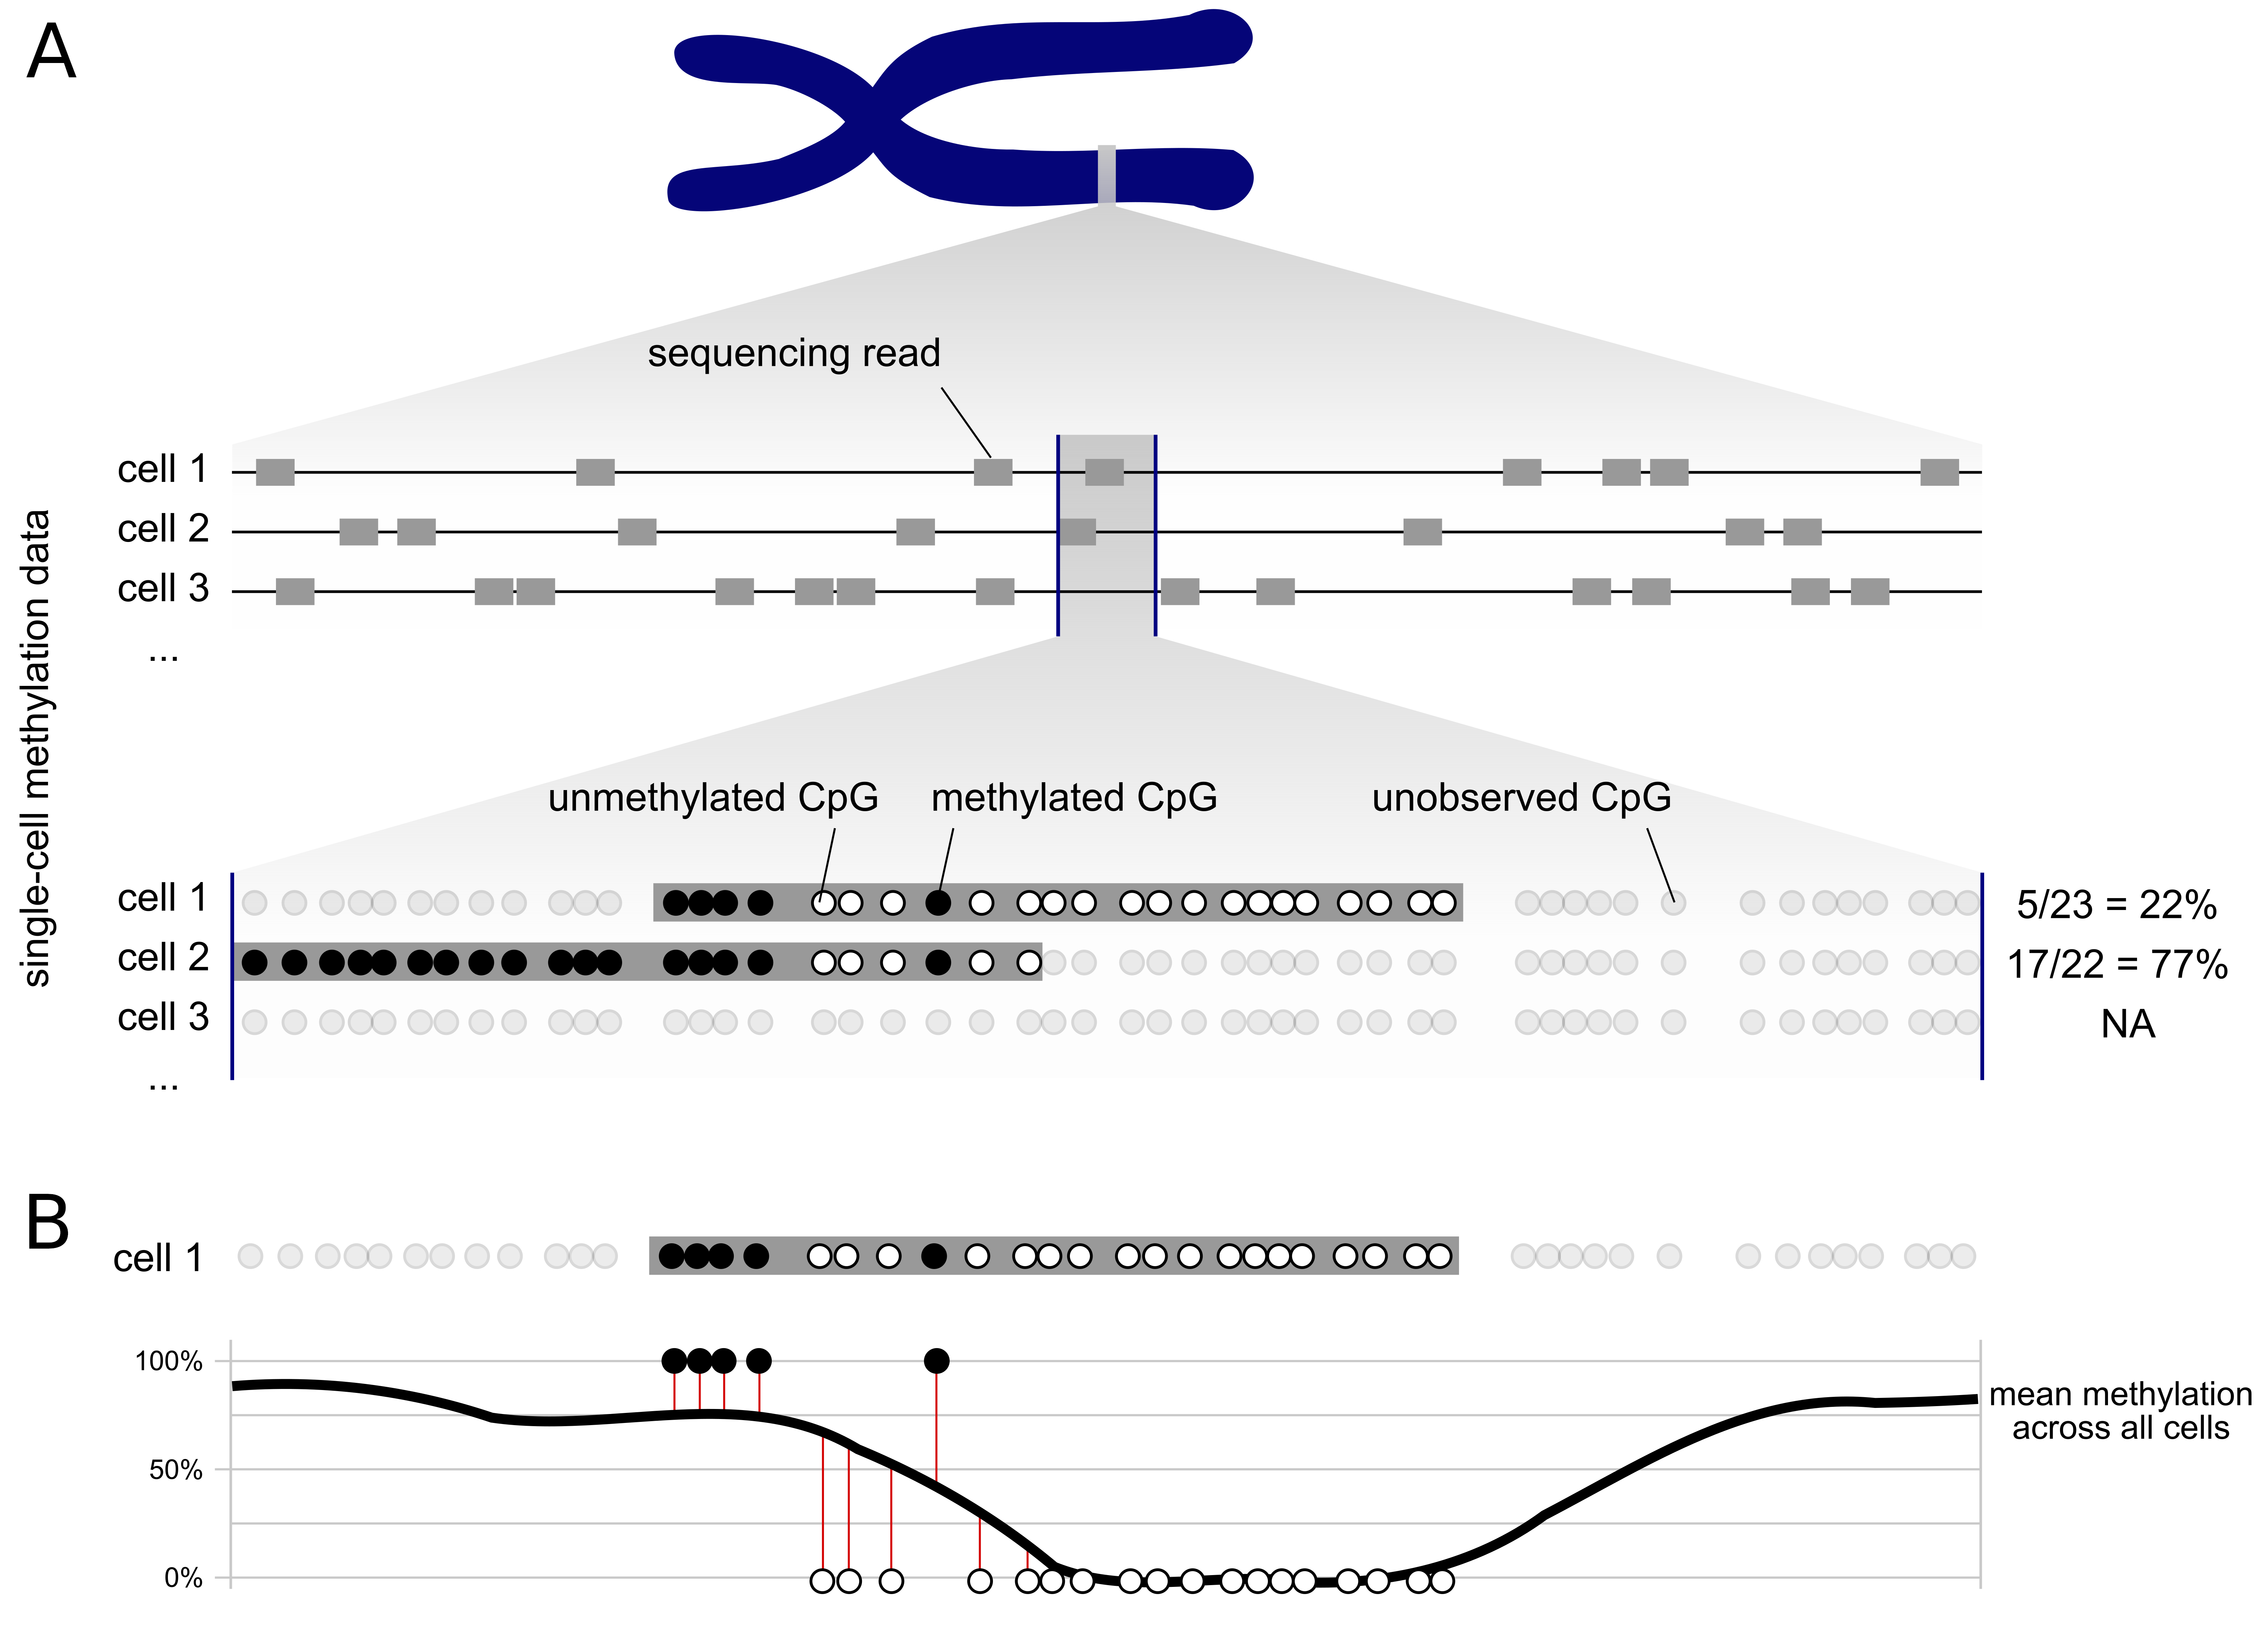
\includegraphics[width=0.7\textwidth]{figures/Fig_residuals_AB.png}\\
    \end{center}
    \caption{\small \textbf{Improved quantification of DNA methylation in a given genomic interval.}\\
    \textbf{(A)} Depicted is a genomic interval (between vertical blue lines) along a chromosome, for which DNA methylation is to be quantified.
    Two cells cover differing parts of the interval with one read each.
    If one simply counts for each cell which fraction of the covered CpG sites are methylated, one obtains very different values for the two cells.
    \textbf{(B)} By averaging each CpG site's methylation over all cells and subsequent smoothing, the thick black ``average methylation curve'' is obtained.
    To quantify the methylation of cell 1 from (A) relative to this average over all cells, we propose to use the cell's residuals to the smoothed curve (lengths of the vertical red lines) and take their average, counting residuals of methylated CpGs positive and residuals of unmethylated CpGs negative.}
    \label{fig:smoothres}
\end{figure*}


The standard approach to analyze scBS-seq data is based on methodology developed for the analysis of scRNA-seq data.
Therefore, we start by briefly reviewing how sc\emph{RNA}-seq data is commonly analyzed, before we discuss scBS data analysis.

The starting point in most scRNA-seq analyses is a matrix of UMI counts (i.e.
of counts of distinct RNA molecules), one row for each cell and one column for each gene.
A first goal is usually to assign cell types or states to cells.
To this end, one needs to establish which cells are similar to each other, i.e., quantify the distance (i.e., dissimilarity) between any two given cells' transcriptional profile.
A standard approach, used with minor variation in virtually all recent research and automated by popular software such as Seurat \citep{Hao_2021} or ScanPy \citep{Wolf_2018}, is as follows: One first accounts for cell-to-cell variation in sequencing depth by dividing each UMI count by the respective cell's total UMI count, then transforms to a homoskedastic scale by taking the logarithm.
In order to avoid matrix elements with zero count to be transformed to minus infinity, one typically adds a very small ``pseudocount'' (often $10^{-4}$) to the normalized fractions before taking the logarithm.
Now, one could use Euclidean distances of these vectors of logarithmized fractions as dissimilarity score.
However, these scores would be exceedingly noisy due to the strong Poisson noise introduced by the many genes with very low counts.
Therefore, one performs a principal component analysis (PCA), keeping only the top few (typically, 20 to 50) components.
As Poisson noise is uncorrelated between genes, it will average out in the top principal components, as these are all linear combinations with weight on a large number of genes.
Therefore, Euclidean distances between these ``PCA space'' vectors provide a robust dissimilarity score.
Hence, the PCA space representation is suitable as input to methods like t-SNE and UMAP, which provide a two-dimensional representation of the data, or to methods for clustering (assigning cells to groups by similarity) and trajectory finding (identifying elongated manifolds in PCA space and assigning cells to quasi-1D positions along them).

This procedure is commonly adapted when working with single-cell DNA methylation data, because once on gets to the PCA step, one can then continue with the established methods just mentioned. The task is therefore to construct from the methylation data a matrix suitable as input for PCA.
A simple and common approach, used for instance by \citet{luo2017single}, is to divide the genome into tiles of e.g. 100~kb size, and calculate for each cell the average methylation of the DNA within each tile.
To this end, one identifies in the tile all CpG sites that are covered by at least one read and averages their methylation state, i.e., one denotes the as average DNA methylation of the tile in a given cell the proportion of the observed CpG sites in the tile that were found to be methylated (Figure \ref{fig:smoothres}A).
This yields a matrix, with one row for each cell and one column for each genomic tile, comprising numbers (``methylation fractions'') between 0 and 1.
This matrix is now subjected to PCA.
After PCA, one can proceed with dimensionality reduction and clustering approaches known from scRNA-seq.

While this simple procedure is straight-forward and produces useable results, it is not optimal. In this paper, we discuss weaknesses of the simple approach and suggest several refinements to overcome them. Using benchmarks and application to real data, we show that our improvements substantially increase the information content of the processed data. In the main text, we explain the proposed methods and their motivation in a qualitative manner, while mathematical details are given later in the Methods section. Then, we will demonstrate the value of our methods using benchmarks and application to real data. Finally, we describe and demonstrate an approach to detect differentially methylated regions (DMRs) in scBS data. We also describe our software toolkit, scbs, that facilitates all these analyses.

\section{Improved preprocessing of scBS data}

%\phantomsection
\subsection{Read-position aware quantitation} \label{residuals}

We first discuss the task of quantifying the level of methylation in a given, fixed, genomic interval. Typically, read coverage per cell is sparse in scBS data. In the example of Figure \ref{fig:smoothres}A, teh depicted interval is covered by a single read for two of the three cells shown and no read in the third. The read from cell 2 shows much more methylation than the read from cell 1, and the standard analysis would therefore consider cell 1 to have higher methylation in the interval than cell 2.
However, given that the two reads agree wherever they overlap, a more parsimonious interpretation would be that the cells do not show difference in methylation within the interval.
Rather, both cells, and similarly maybe most other cells, might have stronger methylation in the left third of the interval than in the middle one.

Therefore, we propose to first obtain, for each CpG position, an average of the methylation across all cells, and then quantify each cell's deviation from this average.
In Figure \ref{fig:smoothres}B, the curved line depicts such an average over all cells, and the red vertical lines show an individual cell's deviation from the ensemble average.
We take the lengths of the red lines as signed values (``residuals''), positive for lines extending upwards from the curve (methylated CpG) and negative for lines extending downwards (unmethylated CpG). For each cell, we then take the average over the residuals for all the CpGs in the interval that are covered by reads from this cell.
In this average, we perform shrinkage towards zero via a pseudocount (to trade bias for variance, see Methods for detail) in order to dampen the signal in cells with low coverage of the interval.

The average thus obtained, the shrunken mean of the residuals, is what we use to quantify the cell's (relative) methylation in the interval.
For a genome tiled into such intervals, we thus obtain a matrix, one row per cell, one column per interval, that can be used for downstream analysis, e.g., as input for PCA.
The signal-to-noise ratio in this matrix will be better than in a matrix obtained by simply averaging absolute methylation (0 or 1) over all the cells' covered CpG sites in a region.
The reason for this is that we reduce the variation in situations as the one depicted in Figure \ref{fig:smoothres}A, where the methylation of the reads might differ strongly even though there is no actual evidence for a difference between the two cells.

How should one obtain the ensemble average (the curved line in Fig.~\ref{fig:smoothres}B)?
A simple approach to get a value for a specific CpG would be to take all cells with read coverage for the CpG and use the fraction of these that show the CpG as methylated.
However, especially when only few cells offer coverage, these averages will be very noisy.
Therefore, we propose to smoothen using a kernel smoother, i.e., by performing a kernel-weighted average over the CpG site's neighborhood.
The kernel bandwidth (i.e., the size of the neighborhood to average over) is a tuning parameter; for the examples presented here we used 1000~bp.

A minor remaining issue is how to deal with the case that a cell has no reads at all within a given interval. Here, it is justified to simply put zero into the matrix element, because a shrunken residual average of zero indicates that there is no evidence of the cell deviating from the mean. We slightly refine this by using an iterative imputation within the PCA (see Methods for details).

Taken together, this shrunken mean of residuals quantitation reduces variance in comparison to simple averaging of raw methylation calls. We will show further below how this improves results.

\subsection{Finding variably methylated regions}

\begin{figure}
    \begin{center}
    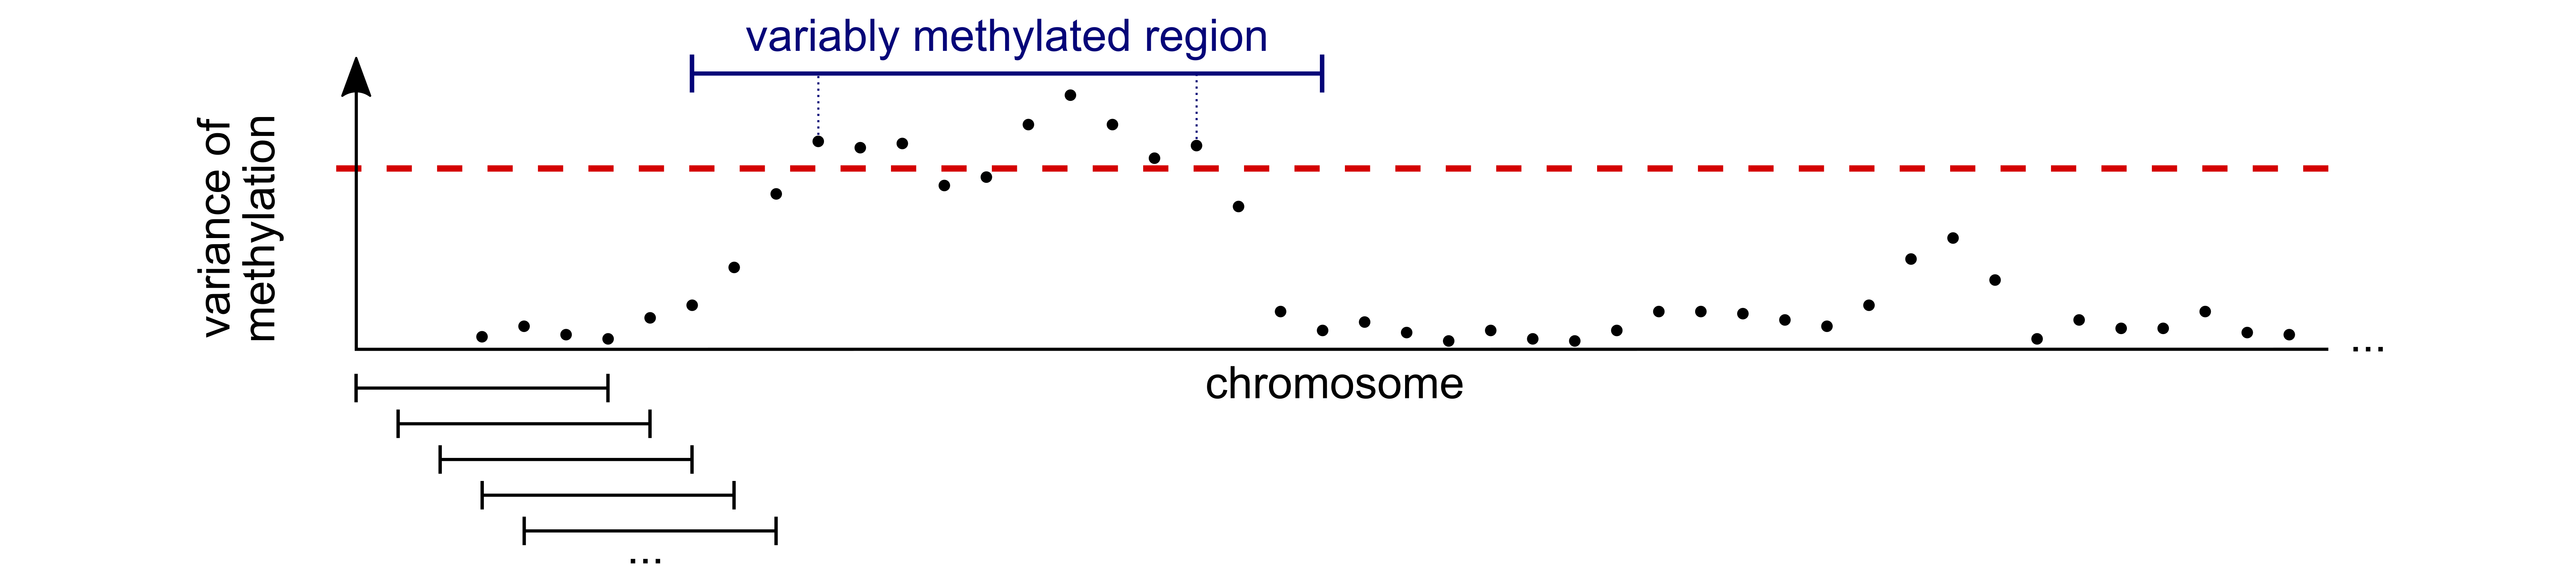
\includegraphics[width=\columnwidth]{figures/Fig_sliding.png}
    \end{center}
    \caption{\small \textbf{Finding variably methylated regions.}\\
    The chromosomes are divided up into overlapping windows (first five shown at the bottom), and for each window, the cells' methylation values are calculated as described and as depicted in Fig.~\ref{fig:smoothres}B.
    Then, the variance of these values is calculated (each point represents one of the overlapping windows), a threshold (dashed line) is chosen such that a chosen quantile of windows have a variance exceeding the threshold.
    Windows with above-threshold variance are merged if they overlap, yielding the ``variably methylated regions'' (VMRs).}
    \label{fig:vmr}
\end{figure}

Typically, some regions in a chromosome will have very similar methylation status in all cells, while other regions show variability in methylation across cells.
For instance, it is known  since long that CpG-rich promoters of housekeeping genes are unmethylated, and that a large proportion of the remaining genome is highly methylated regardless of cell type \citep{bird1986cpg}.
In contrast, DNA methylation at certain genomic features such as enhancers is more dynamic (e.g., \citet{argelaguet2019gastru}), and thus more variable across cells.
Only the latter regions are of value for our goal of quantitating dissimilarity between cells.
We call these the variably methylated regions (VMRs). % maybe mention the parallel to highly variable genes in scRNAseq?

In the standard approach, one divides up (tiles) each chromosome into non-overlapping, equal-sized intervals, and quantitates the methylation of each tile.
Such rigid placing of interval boundaries is unlikely to be optimal: for example, a VMR might be much smaller than a tile and the signal from its CpG sites will hence be drowned out by the larger number of uninformative CpG sites that are equal in all cells, when averaging over all the CpG sites in the tile.

Therefore, we propose the following approach (Fig.~\ref{fig:vmr}): Divide up the chromosome into many \emph{overlapping} windows that start at regular multiples of a fixed, small, step size.
Quantify the methylation of each cell in each window by averaging the cell's methylation residuals over all CpGs in the window, as described above and depicted in Fig.~\ref{fig:smoothres}B.
Then, calculate for each window the variance of these values over all cells.
Select, say, the top 2\% windows with the highest variances and mark them as VMRs.
Wherever thus marked windows overlap or are separated by only a small gap, merge them into one larger VMR.
Then, calculate for each of these larger VMRs the methylation signal, as before, by averaging for each cell over the residuals of all contained CpG sites.

In this manner, we obtain a methylation matrix, with one row per cell and one column per VMR, that is, in a sense, richer in information and has better signal-to-noise ratio than the matrix obtained by the simple analysis sketched at the very beginning.
As we demonstrate below, a PCA performed on such a matrix provided a distance metric for the cells that contains more information on biological detail than one from a simpler analysis.

\begin{figure*}
	\begin{center}
		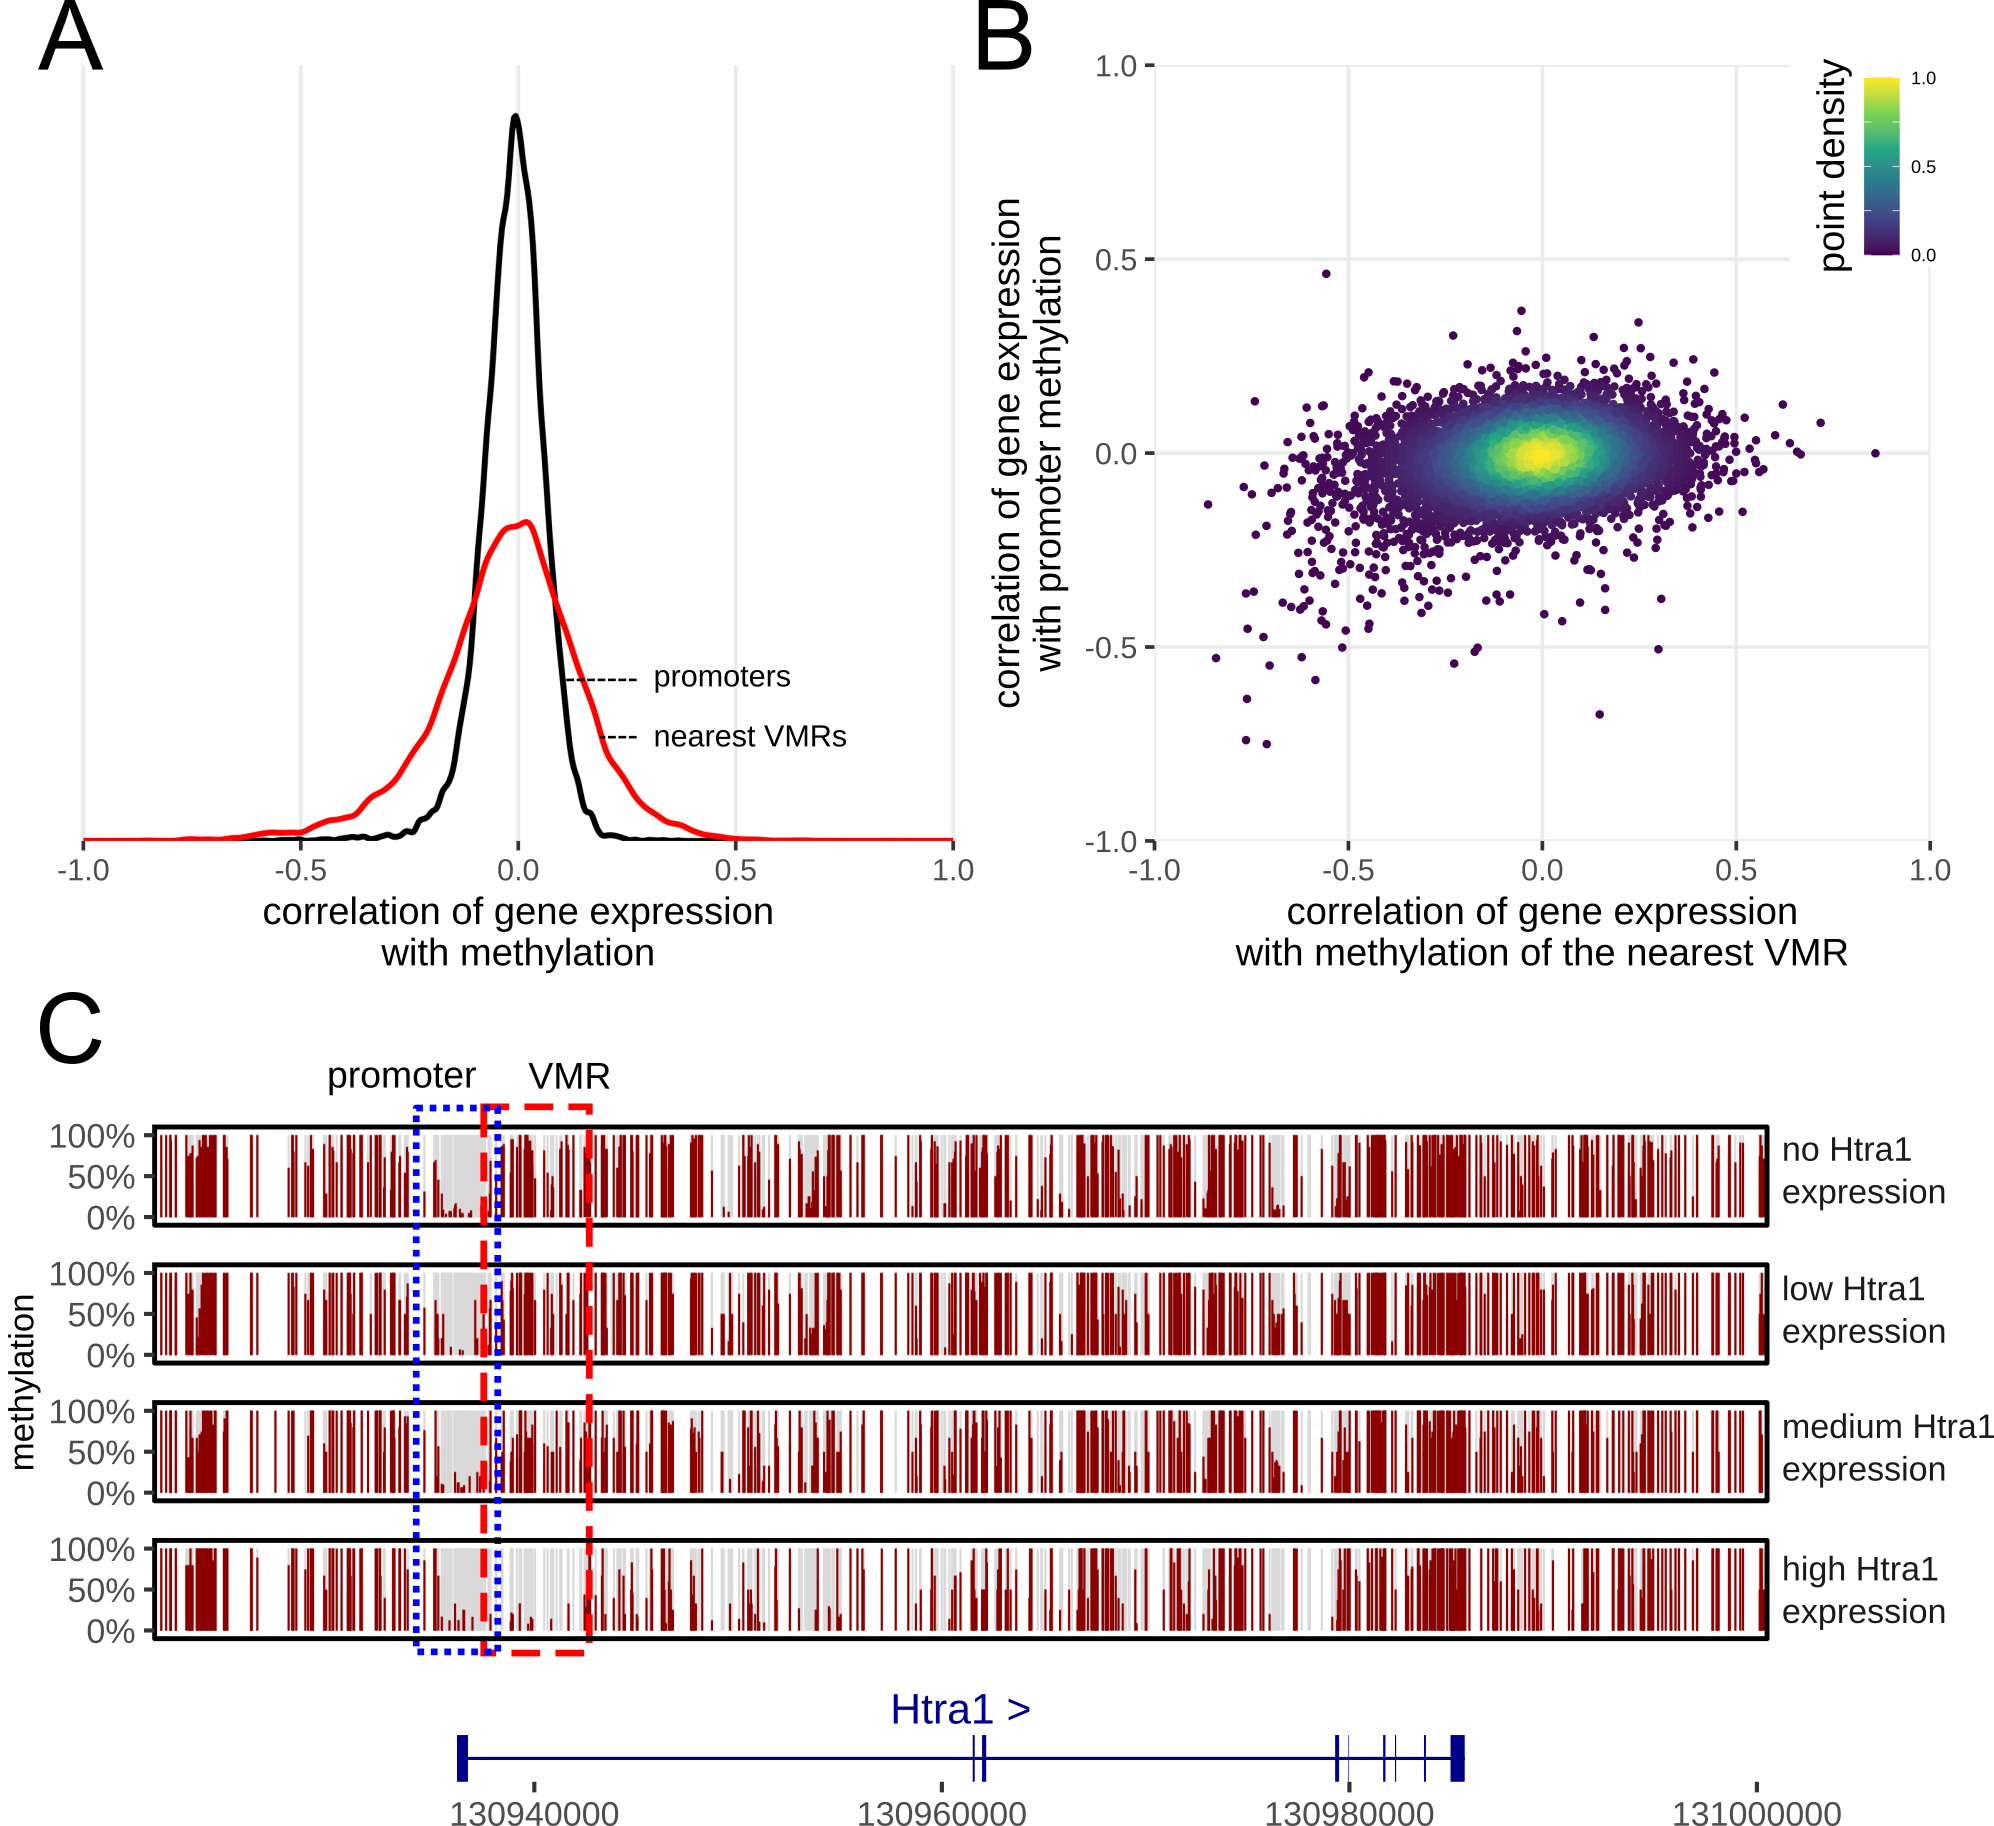
\includegraphics[width=\textwidth]{figures/Fig_correlation.png}
	\end{center}
	\caption{\small \textbf{Correlation of DNA methylation and gene expression}.\\
		\textbf{(A)} Distribution of Pearson correlations between gene expression and promoter methylation (black) and gene expression and methylation of the nearest VMR (red): for most promotors, correlation is weak. Promoters are defined as intervals \textpm2~kb around the TSS.
		\textbf{(B)} Mean methylation near the gene Htra1.
		Cells are assigned to 4 groups based on Htra1 expression (group 0: cells with no Htra1 expression, groups 1-3: cells that express Htra1, divided into three equally large groups with group 3 having the highest expression).
		Data from \citet{kremer_scnmt}.}
	\label{fig:correlation}
\end{figure*}

\begin{figure*}
	\begin{center}
		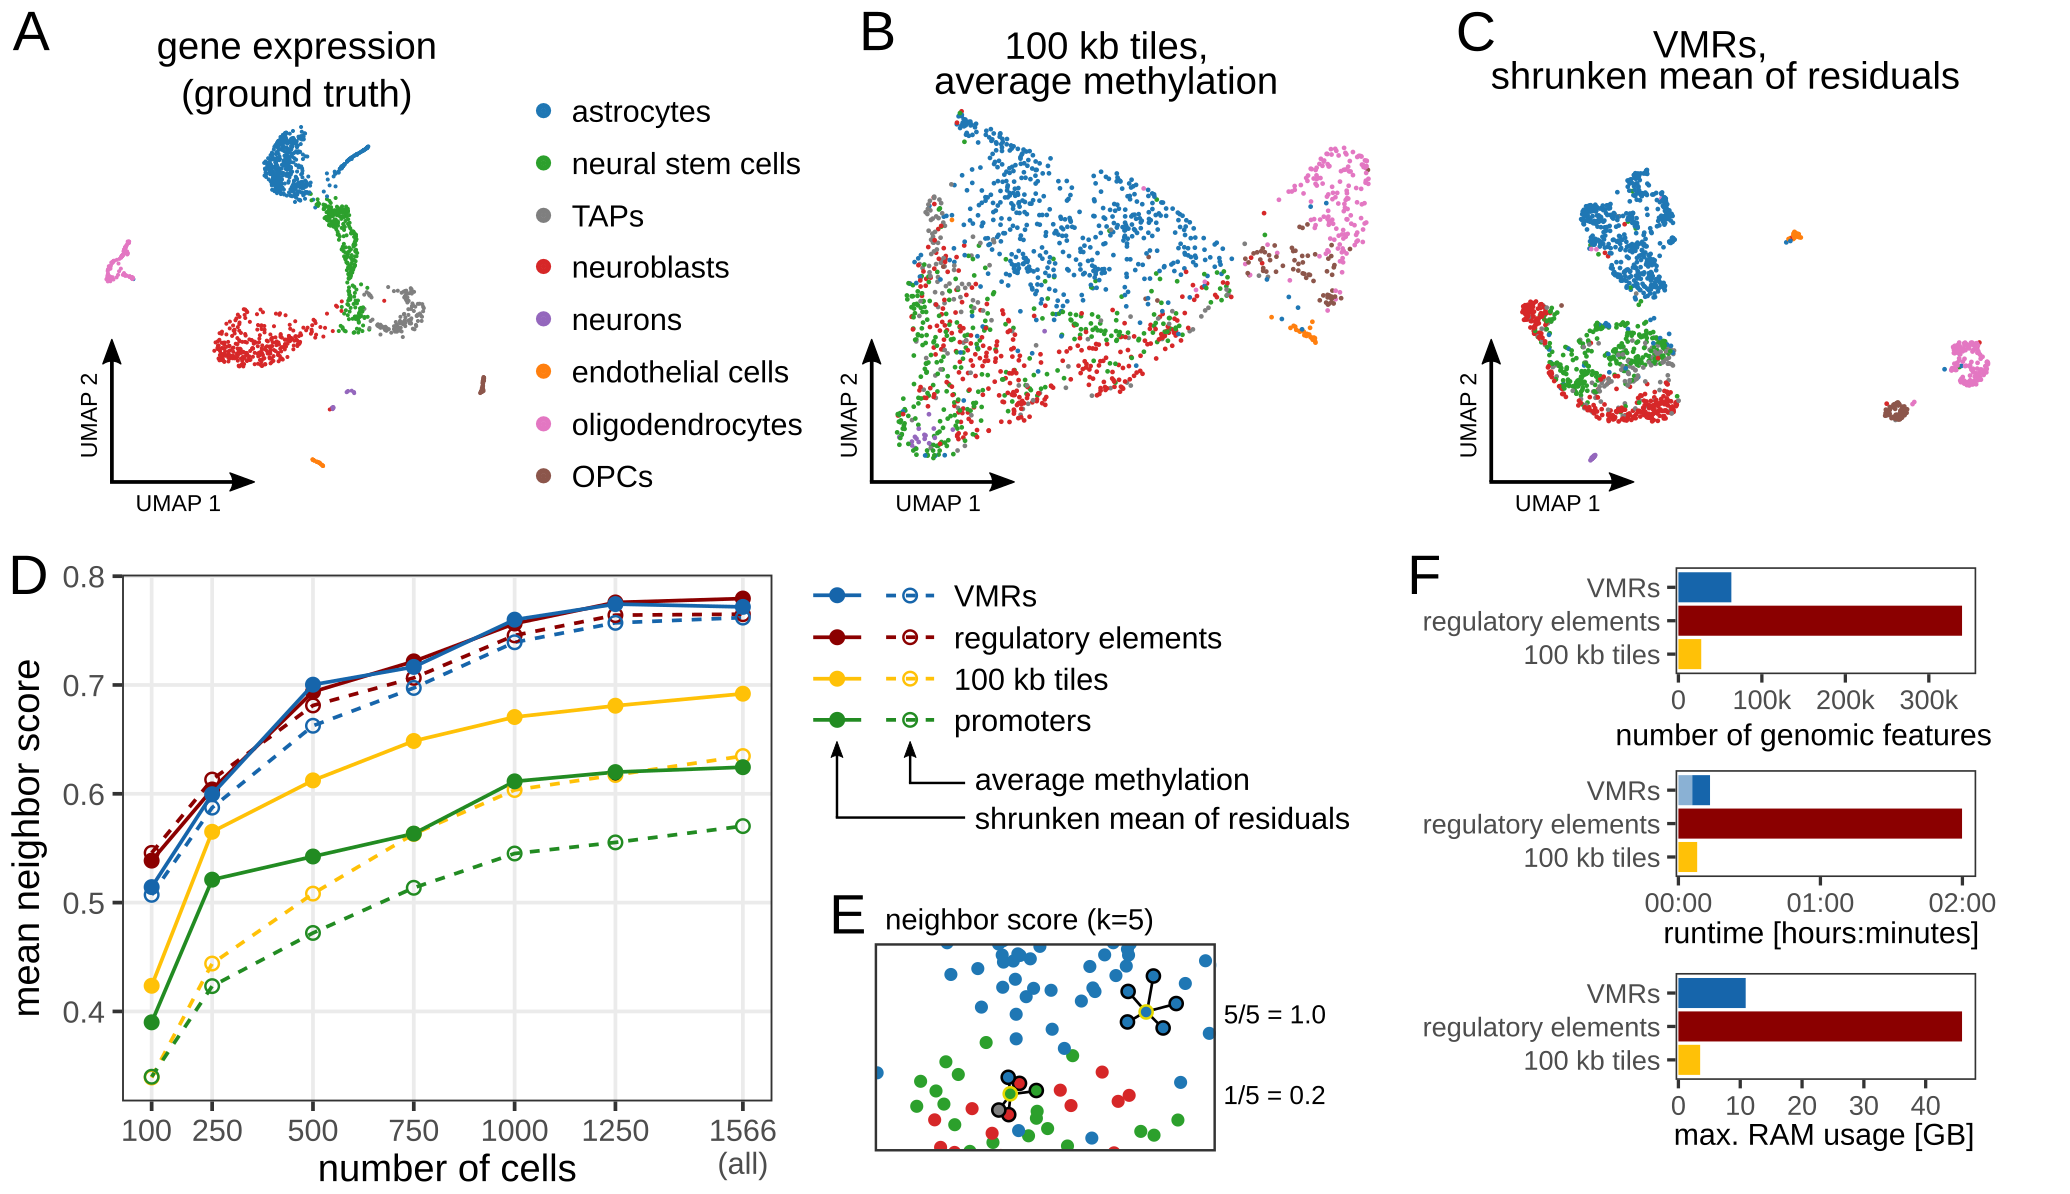
\includegraphics[width=0.8\textwidth]{figures/Fig_benchmark.png}
	\end{center}
	\caption{\small \textbf{Benchmark of our methods on single-cell multi-omic data of cells of the murine forebrain}.\\
		\textbf{(A)} Cell labels based on clustering of single-cell transcriptomes from \citet{kremer_scnmt}.
		\textbf{(B, C)} Exemplary UMAPs obtained when analyzing the data set with our proposed methods (B) or conventional methods based on genome tiling (C).
		\textbf{(D)} Illustration of the neighbor score. Note that, actually,
		distances are measured in 15-dimensional PC space, not in the 2-dimensional
		UMAP space.
		\textbf{(E)} Mean neighbor score obtained after analysing single-cell methylomes with different combinations of methods.
		Either 100~kb genomic tiles or VMRs were subjected to PCA and UMAP.
		Tiles or VMRs were pre-processed as proposed in this work (shrunken mean of residuals subjected to iterative PCA) or using conventional methods (PCA on methylation percentages, lightly imputed as done in \citet{luo2017single}; see Methods for details).
		The full 1566-cell data set was sub-sampled to simulate smaller data sets (x axis).
		A higher neighbor score implies better separation of cell types inferred from single-cell transcriptomes of the same cells \textbf{(A)}.
	}
	\label{fig:score}
\end{figure*}


\subsection{Application and benchmarks}

To demonstrate the value of our proposed improvements, we employ our own data \citep{kremer_scnmt} as well as a previously published data set, namely the one by  \citet{luo2017single} already mentioned in the introduction.

%\phantomsection
\subsubsection{Correlating VMR methylation with gene expression}

Our data set \citep{kremer_scnmt} comprises the methylomes of 1566 cells isolated from mouse forebrains, as well as matched single-cell transcriptomes of the same cells.
Among these cells are distinct cell types such as oligodendrocytes, oligodendrocyte precursor cells (OPCs) and endothelial cells, as well as cellular sub-states that are part of the continuous neural stem cell differentiation trajectory.
To assess whether our VMR detection method captures genomic intervals that are biologically meaningful, we probed whether their methylation level correlates with the expression of nearby genes.

We first note that gene expression is more strongly correlated with the methylation of nearby VMRs than with the methylation of their promotors (Fig.~\ref{fig:correlation}A), indicating that VMR methylation is often a better predictor of gene expression than promoter methylation.
Indeed, a gene-wise comparison revealed many genes whose expression is correlated with the nearest VMR, but not with promoter methylation (Fig.~\ref{fig:correlation}B).
One such example gene, Htra1, is depicted in Fig.~\ref{fig:correlation}C.
While the promoter of this gene is lowly methylated regardless of gene expression, a VMR located downstream of the promoter is lowly methylated in cells with high Htra1 expression.

\subsubsection{Improved identification of cell types}

We next tested whether our methods improve the ability to distinguish cell types and cell states (Fig.~\ref{fig:score}).
To this end, we obtained cell type/state labels based on the single-cell transcriptomes from \citet{kremer_scnmt} (Fig.~\ref{fig:score}A).
We consider these cell labels as ground truth and tested whether we are able to distinguish the same groups of cells based on their methylomes.
To do this, we subjected the methylomes to four variants of the workflow described above: we defining genomic intervals in two ways and quantified methylation in these intervals in two ways, then always subjected the resulting matrix to PCA.
To define the intervals, we either simply tiled the genome into 100~kb bins as is commonly done, or we used our VMR detection approach.
To quantify methylation in these intervals, we either averaged in these intervals, obtaining methylation percentages (``classic'' pre-processing), or we calculated the shrunken mean of residuals.

Visual inspection of the resulting UMAPs revealed that our proposed combination of methods results in more clearly separated cell types, compared to a UMAP obtained with default analysis methods (Fig.~\ref{fig:score}B,C).
While all cells form a continuous point cloud when using default methods, our improvements led to a clear separation of oligodendrocytes, OPCs and endothelial cells.
Furthermore, even cellular sub-types of cells in the continuous neural stem cell lineage were partially separated.

To quantify this performance gain in a more rigorous manner, we used a score that quantifies whether cells were placed, in 15-dimensional PC space, in a neighborhood comprising cells of the same cell type ("neighbor score", see Figure \ref{fig:score}D, and Methods for details).
We then ask how this score depends on the number of available cells. This is relevant as scBS protocols are costly and labor-intensive, and only few laboratories are currently able to obtain thousands of single cell methylomes. To simulate smaller data sets, we sub-sampled the 1566-cell data set into smaller data sets, analyzed them again with the four workflow variants, and calculated the mean neighbor score for each (Figure \ref{fig:score}E).
The results demonstrate that the forebrain cell clusters are more cleanly separated when using our proposed methods.
This performance gain was observed also in smaller data sets, although cell cluster separation generally becomes more difficult in those.
Both the use of VMRs instead of genomic tiles, as well as the use of the shrunken mean of the residuals over methylation averages improved cell cluster separation.

We repeated this benchmark on the data set published by \citet{luo2017single}, which consists of 3377 single-cell CpG methylomes from the murine frontal cortex, comprising 16 neuronal subtypes.
The authors annotated cell types based on CH-methylation instead of CpG-methylation.
Using these labels as ground truth we re-analyzed the full and sub-sampled CpG methylation data with the four methods combinations and found that our suggested methods consistently outperformed default methods (Fig.~\ref{fig:score_luo}).

\subsubsection{Robustness to parameter changes}

Lastly, we assessed whether our proposed workflow requires fine-tuning of parameters (Fig.~\ref{fig:sweep}).
To this end, we re-analyzed both data sets, as well as sub-samples of the data with different VMR detection parameters, namely the width of the sliding window in bp, (set with option \texttt{--bandwidth} in our ``scbs'' software, default 2000 )and the variance threshold above which windows are merged to VMRs (\texttt{--var-threshold}, default 0.02).
This parameter sweep showed that our workflow gives good results over a wide range of parameter values. For the data of \citet{luo2017single}, results are nearly independent of the parameters (Fig.~\ref{fig:sweep}B). In the more challenging data set of \citet{kremer_scnmt} (Fig.~\ref{fig:sweep}A), cell types were less cleanly separated when very large bandwidths, or very strict variance thresholds were selected.
However, very small bandwidths or very lenient thresholds resulted in a much higher number of VMRs and thus long computing times. Overall, however, our default parameter combination provided good results and fast compute times in both data sets.

\begin{figure*}
	\begin{center}
		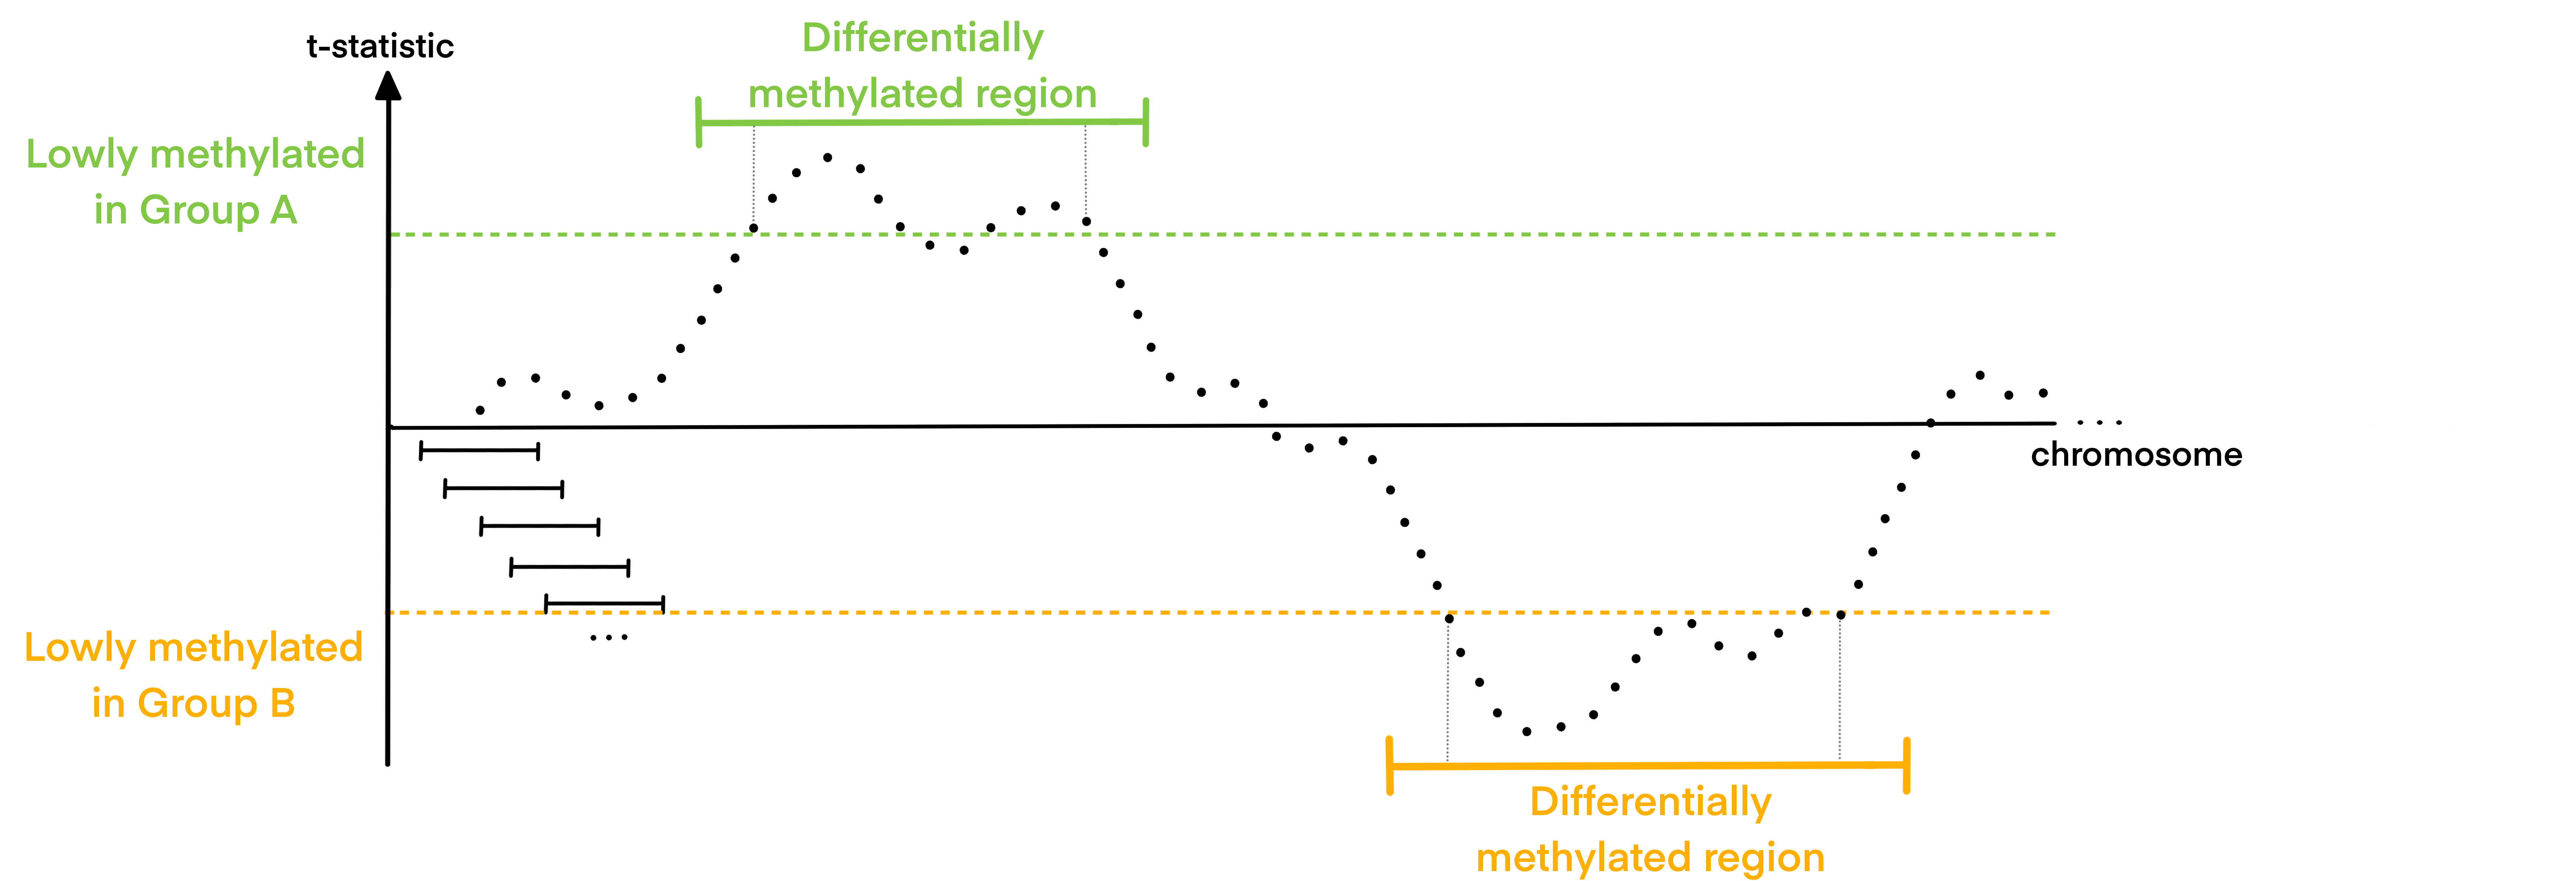
\includegraphics[width=.75\textwidth]{figures/Fig_DMRdetection.png}
	\end{center}
	\caption{\small \textbf{Identification of differentially methylated regions.}\\
		The chromosome is divided into windows overlapping by a small and fixed size.
		For each window, the cell’s methylation values are calculated as described and as depicted in Fig.~\ref{fig:smoothres}B.
		Then the t-statistic of these values is obtained as a measure of methylation difference (each point represents one of the windows).
		Upper and lower thresholds (dashed lines) are chosen such that a defined quantile of windows have a t-statistic above or below the threshold.
		Windows exceeding either threshold are merged if they overlap, yielding the differentially methylated regions (DMRs).}
	\label{fig:dmrscan}
\end{figure*}



\section{Finding differentially methylated regions}

A common task in the analysis of bulk bisulfite-sequencing data is the detection of differentially methylated regions (DMRs) between conditions, tissues, or cell types \citep{Hebestreit2013, dmrseq}.
As DNA methylation affects gene expression, DMRs can provide insights into the unique epigenetic and gene regulatory characteristics of cell types.
However, to date no approach to detect DMRs in scBS data has been reported.
To enable DMR detection in scBS data, we thus developed an approach that detects DMRs of variable size between two groups of cells, and controls the false discovery rate (Fig.~\ref{fig:dmrscan}):

Similar to the previously described approach for VMR identification (Fig.~\ref{fig:vmr}), we divide each chromosome into overlapping windows shifted by a small and fixed size (step size) and quantify the methylation of each cell in each window.
Next, instead of the variance, we obtain the t-statistic % Welch t-test
as a measure of differential methylation between the two cell groups.
We identify the windows with the most extreme t-statistics, e.g. windows in the 2\% upper and lower tails. We the merge any overlapping windows in the upper tail into larger DMRs, and do the same for windows in the lower tail, and then we re-calculate the t-statistic for each larger DMR.

To assess statistical significance of DMRs, we repeat the same procedure on permutations of the scBS data, i.e. the same data set with randomly shuffled cell labels. The DMR t-statistics obtained from permuted data are then used to estimate the false-discovery rate (FDR), yielding an adjusted p-value for each DMR.

While the primary purpose of VMRs is to provide better input for PCA and distance calculations, DMR detection facilitates the discovery of epigenetic differences between conditions or cell types, as we demonstrate next.

\begin{figure*}
	\begin{center}
		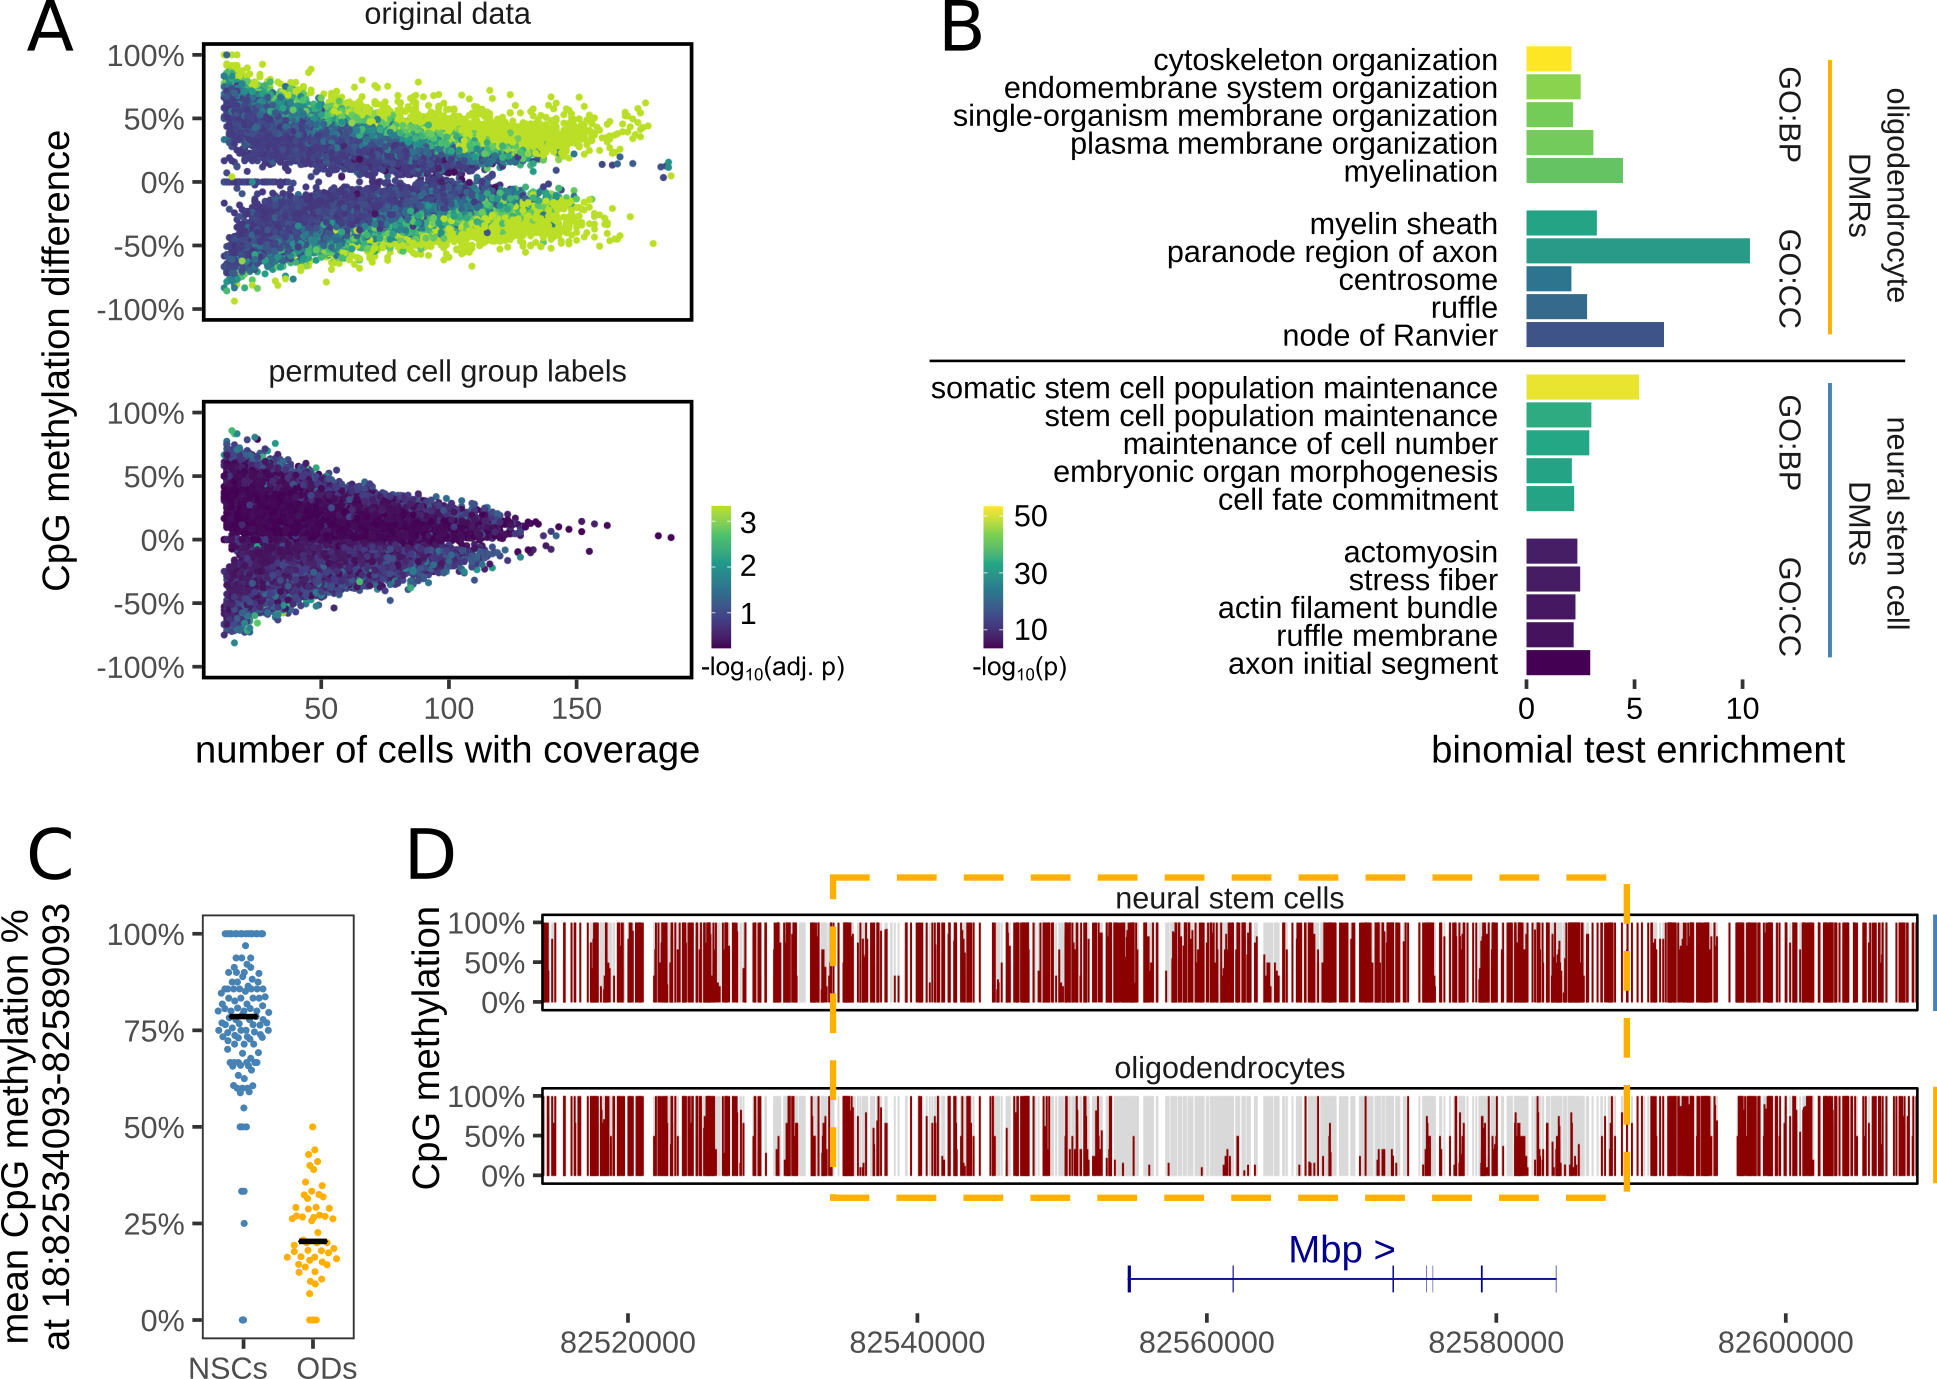
\includegraphics[width=.7\textwidth]{figures/Fig_DMRs.png}
	\end{center}
	\caption{\small \textbf{Detection of differentially methylated regions between oligodendrocytes and neural stem cells.}\\
		\textbf{(A)} DMRs detected between 58 oligodendrocytes (ODs) and 130 neural stem cells (NSCs) from \citep{kremer_scnmt} (top) and DMRs detected in the same data with randomly permuted cell labels (bottom, used to estimate FDR and determine adjusted p-values).
		\textbf{(B)} Enrichment of GO terms associated with DMRs lowly methylated in ODs (top) or NSCs (bottom).
		Depicted are the top 5 GO terms of the "Biological Process" (GO:BP) and "Cellular Component" (GO:CC) GO category, and their binomial test p-value and enrichment, as reported by GREAT \citep{mclean2010great}.
		\textbf{(C)} Mean methylation of NSCs and ODs at an exemplary DMR.
		Each point corresponds to a cell, black lines denote the median.
		\textbf{(D)} Detailed view of the DMR (yellow dashed rectangle) from \textbf{C} in pseudo-bulk samples consisting of NSCs or ODs.
		Vertical bars represent CpG sites.
	}
	\label{fig:dmr}
\end{figure*}

%\phantomsection
\subsection{Detecting DMRs between oligodendrocytes and neural stem cells}


We used the single-cell multi-omics data set \citep{kremer_scnmt} to evaluate our DMR detection approach.
We first selected two cell populations from the healthy murine ventricular-subventricular zone: neural stem cells (NSCs, 130 cells) and oligodendrocytes (58 cells).
Then we used the method just described to identify DMRs between these two cell types (Fig.~\ref{fig:dmr}A). Repeating this after permuting the cell-type labels, in order to obtain a null distribution fo the t statistics, yielded
DMRs with much weaker methylation differences. Consequently, we could assign to many of the DMRs detected in the unpermuted data a low adjusted p-values (colours in Fig.~\ref{fig:dmr}A).

Gene ontology (GO) enrichment with GREAT \citep{mclean2010great} revealed that DMRs lowly methylated in oligodendrocytes are located near genes involved in myelination, the main function of oligodendrocytes.
Similarly, DMRs specifically demethylated in NSCs occur near genes involved in stem cell population maintenance.
This demonstrates that our DMR detection approach is able to identify biologically meaningful DMRs, even in scBS data sets of modest cell number.

Fig.~\ref{fig:dmr}C-D depicts an exemplary DMR, located at the gene body of myelin-basic protein (Mbp), the major component of myelin that is essential for myelination of neuronal axons \citep{mbp}.
Our results suggest that oligodendrocyte-specific gene expression of Mbp is supported by low methylation at the detected DMR.


\section{The \texttt{scbs} software toolkit}

\begin{figure*}[t]
    \begin{center}
        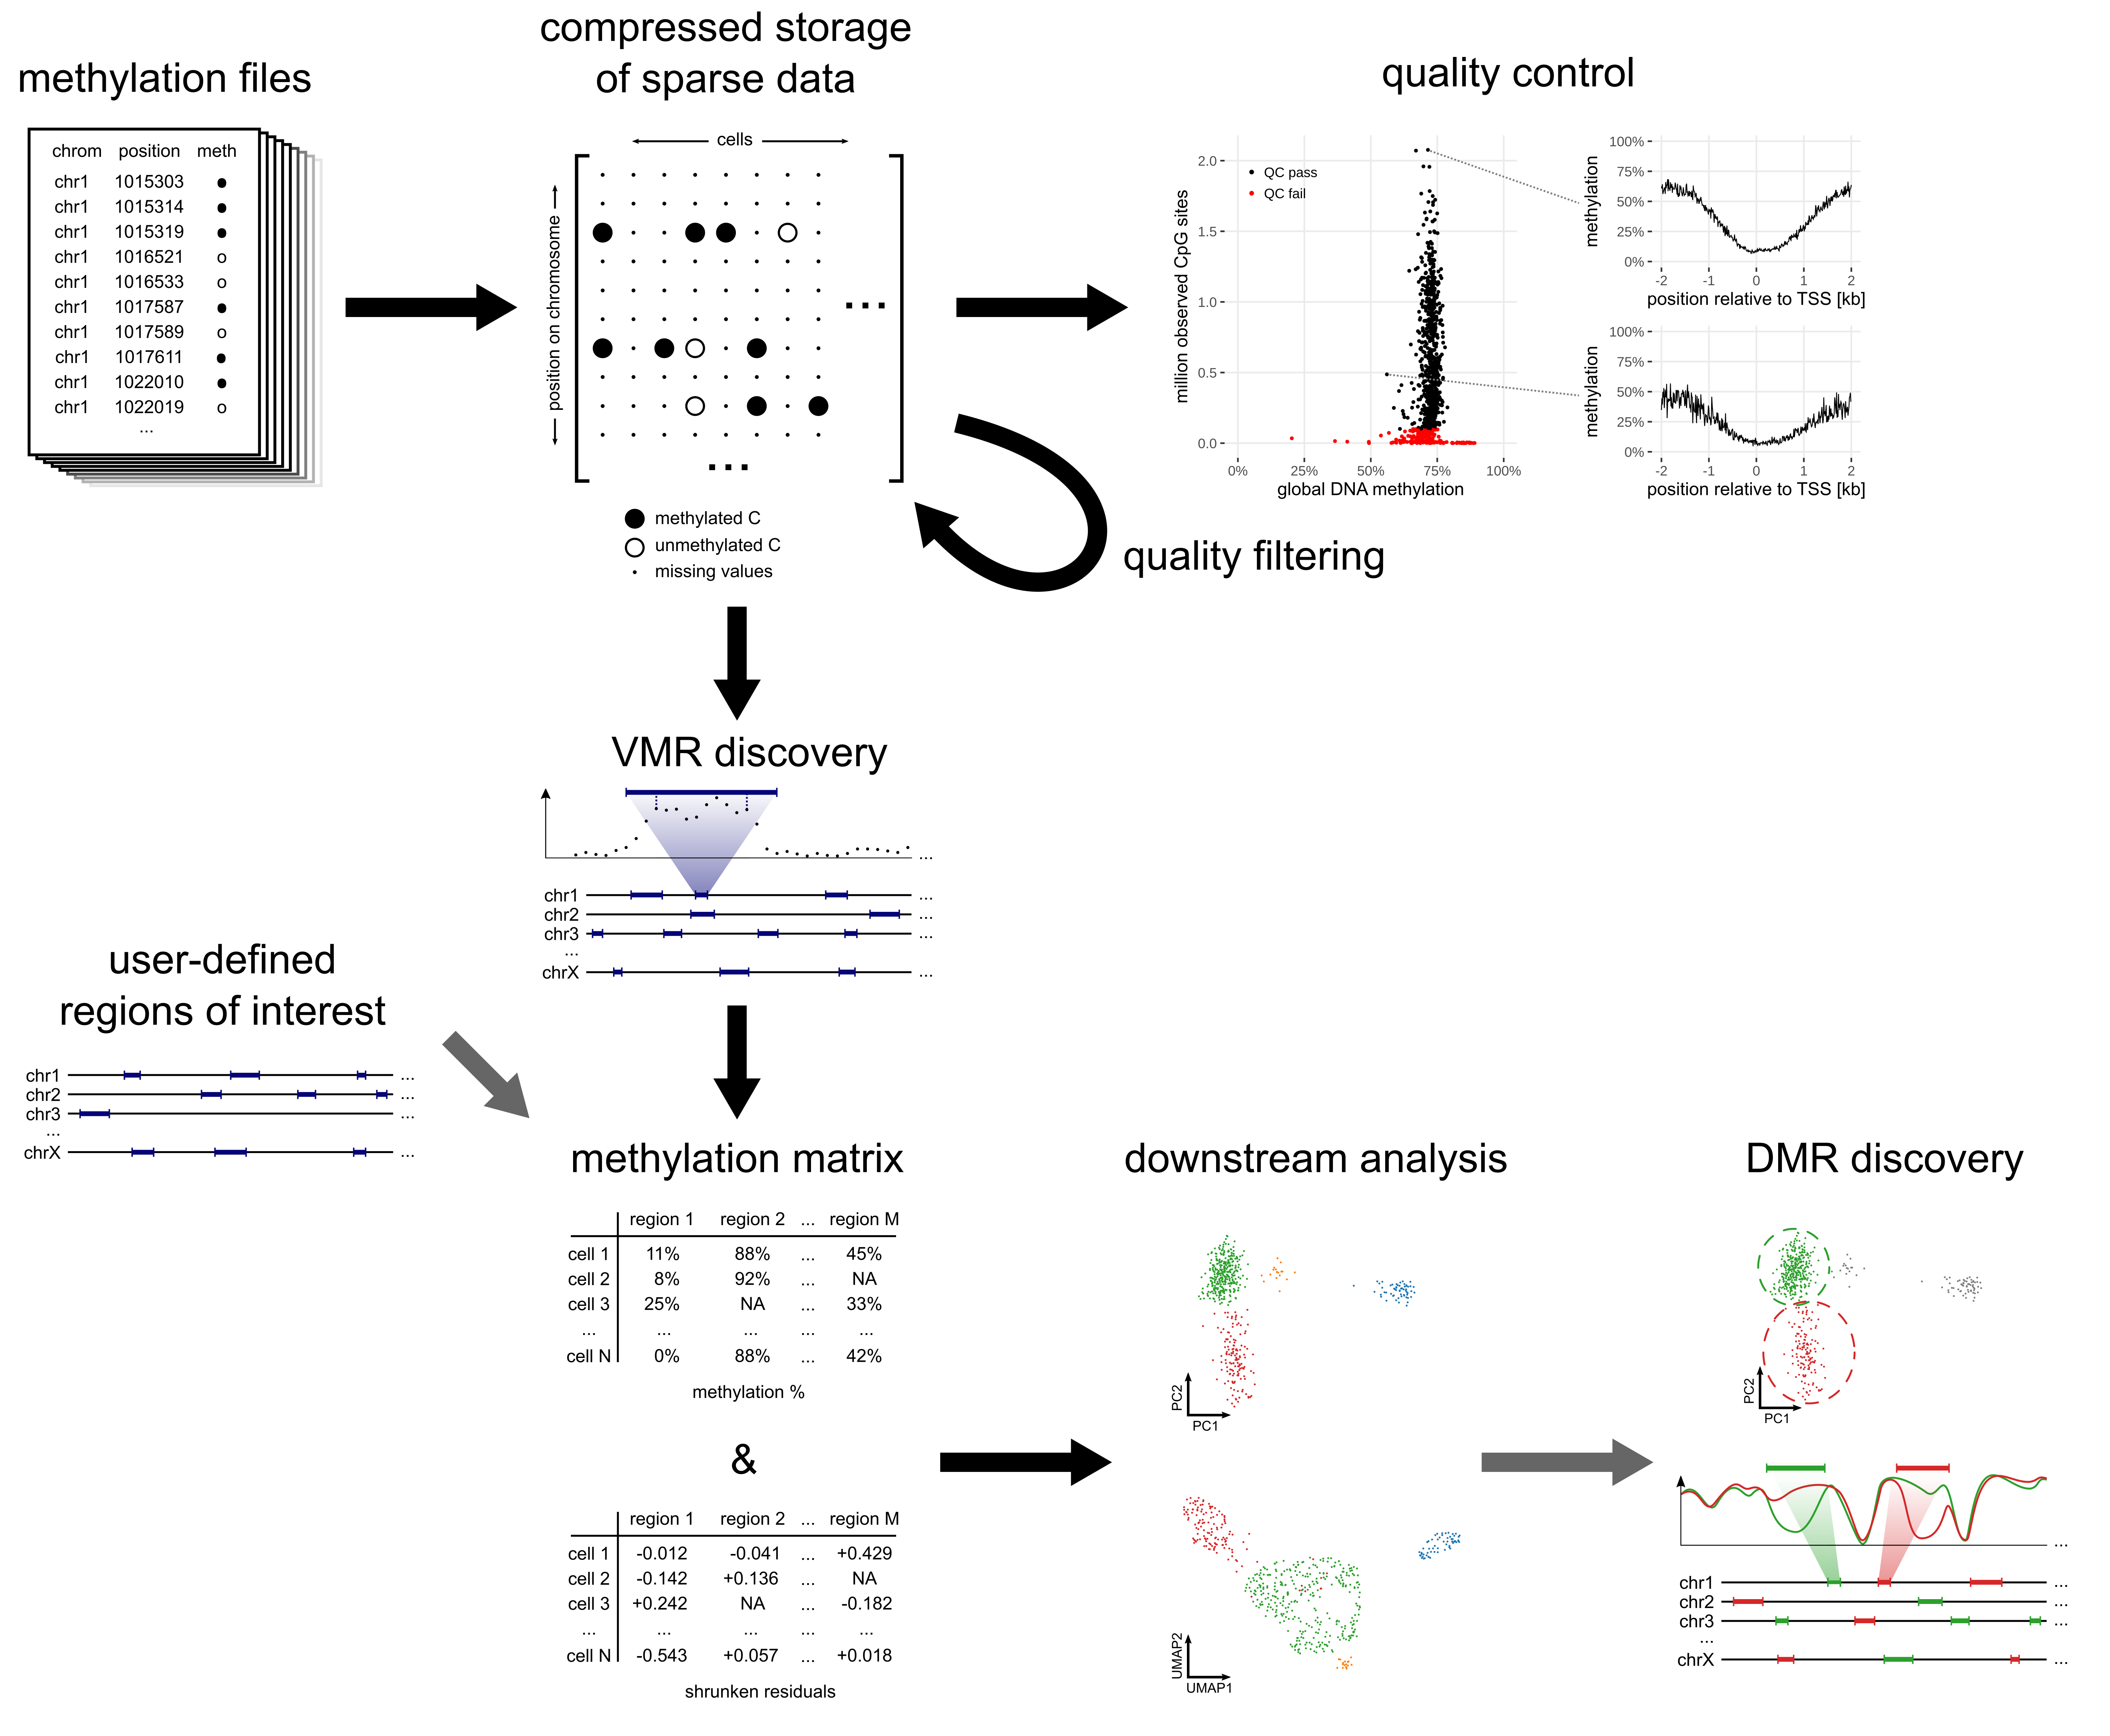
\includegraphics[width=.8\textwidth]{figures/Fig_workflow.png}
    \end{center}
    \caption{\small \textbf{Overview of the functionalities implemented in the \texttt{scbs} package.}\\
        \texttt{scbs prepare} parses methylation files produced by common bisulfite sequencing mappers and stores their contents in a compressed format optimised for efficient access to genomic intervals.
        \texttt{scbs} also produces cell-wise summary statistics and quality plots (here: average methylation around the transcription start site) that are used to detect low-quality cells.
        These cells can be discarded with \texttt{scbs filter}.
        To obtain a methylation matrix, similar to the count matrices used in scRNA-seq, the user must first decide in which genomic intervals methylation should be quantified.
        The user may either provide genomic regions of \emph{a priori} interest, or they may choose to discover VMRs (variably methylated regions) in the data with \texttt{scbs scan}.
        The resulting methylation matrix can then be used for downstream analysis such as cell clustering and dimensionality reduction.
        Identified groups of cells (e.g. clusters) can then be scanned for DMRs with \texttt{scbs diff}.
    }
    \label{fig:workflow}
\end{figure*}

We have implemented the approach just described in a Python package with a command line interface, called \texttt{scbs}, which also offers a number of other functionalities for the analysis of scBS data (Figure \ref{fig:workflow}).
The starting point of such an analysis are methylation files generated by tools such as Bismark \citep{bismark}, methylpy \citep{methylpy} or BISCUIT \citep{biscuit}.
For each cell, these tools produce a text file that lists the methylation status of all CpG sites.
Since it is inconvenient to work with hundreds or thousands of text files, \texttt{scbs} provides the \texttt{prepare} command which parses these methylation files and stores their content in a compressed format that enables efficient access to all CpG sites of the genome.
\texttt{scbs prepare} is flexible and accepts all tabular input formats including Bismark .cov-files, methylpy .allc-files, or custom user-defined formats.

In brief, we store methylation of each chromosome in a matrix where each column represents a cell and each row represents a base pair.
Methylated and unmethylated sites are coded as $+1$ and $-1$, respectively.
Since the vast majority of values in this matrix are missing due to the sparsity of scBS data (and because rows for base-pairs not corresponding to a CpG site contain no data), we encode missing values as zero and then store the data in Compressed Sparse Row (CSR) format.
This format does not explicitly store zeroes (here: missing values) and is optimized for row-wise access, which results in significant compression and allows fast access to the methylation status of genomic intervals.

\texttt{scbs prepare} also computes a number of summary statistics for each cell, including the mean genome-wide methylation level and the number of observed CpG sites, i.e.
the number of CpG sites that have sequencing coverage.
These summary statistics can be used to detect cells with poor quality.
The quality of each single cell methylome can furthermore be inspected with \texttt{scbs profile}, which computes the average methylation profile of a set of user-defined genomic regions such as transcription start sites (TSS) at single-cell resolution.
The TSS profile is a useful quality control plot since methylation shows a characteristic dip roughly \textpm1~kb around the transcription start site in mammalian genomes.
Cells that do not show this pattern, or cells with few observed CpG sites, may then be discarded with \texttt{scbs filter}.


After quality control, the user has access to the genome-wide VMR detection approach described earlier, using the \texttt{scbs scan} command.
This produces a BED file that lists the genome coordinates of VMRs.
To finally obtain a methylation matrix analogous to a scRNA-seq count matrix, this BED file can be used as input for \texttt{scbs matrix}, which quantifies methylation at genomic intervals in all cells.
The command produces both, the simple percentage of methylated CpG sites, as well as our proposed methylation measure, the shrunken mean of the residuals, which is more robust to variation in sequencing coverage or stochastic differences in read position between cells.
We note that both \texttt{matrix} and \texttt{profile} accept any valid BED file as input, which means that the user can quantify and visualize methylation at any set of genomic features of interest, such as promoters, enhancers or transcription factor binding sites, obtaining one profile plot per cell.

The methylation matrix produces by the \texttt{matrix} function can then serve as input for standard single-cell analysis tools like Seurat \citep{seurat} or scanpy \citep{Wolf_2018}, in order to perform, e.g., dimensionality reduction and cell clustering. For this, the methylation matrix should in lieu of the log-normalized expression matrix usually expected by these tools.

Finally, after annotation and exploration of the data set, the user may specify two groups of cells for DMR detection with \texttt{scbs diff}.
This command produces a BED file listing the genome coordinates, adjusted p-values, as well as several other metrics associated with DMRs.
These DMRs may then be associated with nearby genes, or used for GO enrichment with tools such as GREAT \citep{mclean2010great} to enable functional interpretation.


\subsection{Availability}

\texttt{scbs} is free and open source.
The package is available on the Python Package Index (PyPI) and can be installed with the Python package installer \texttt{pip}.
The source code is hosted at \href{https://github.com/LKremer/scbs}{https://github.com/LKremer/scbs}, where we also provide detailed documentation including a tutorial that demonstrates a complete \texttt{scbs} analysis on an example data set.


\section{Discussion and Conclusion}

Here, we have proposed an improved strategy to preprocess single-cell bisulfite sequencing data.
Based on the observation that incomplete read coverage of a genomic interval can lead to inaccurate methylation estimates, we suggest a scoring scheme that is aware of a read's local context rather than just treating all reads in an interval alike.

Furthermore, we show a way to pinpoint minimal regions of high variability across cells, which we call variably methylated regions (VMRs).
By re-analyzing two published data sets, we could show that these improvements to data preprocessing help to increase signal and decrease noise, resulting in a more informative intermediate-dimensional representation of the data.
As examples of practical benefits, we demonstrate that our preprocessing allows for better distinction of cell sub-types, especially for challenging data sets comprising cellular sub-states and lineage transitions or for data sets with small cell number.

To furthermore aid interpretation of scBS data, we developed and implemented the first single-cell DMR detection algorithm.
FDR estimation via permutation allows us to report statistical significance of each DMR.
% maybe here discuss pseudoreplication issues?
Applying our approach to NSCs and oligodendrocytes demonstrated that the obtained DMRs locate near meaningful loci associated with cell-type specific functions.
Thus, our method aids biological interpretability by pinpointing the regions that differ between groups of cells and hence have a putative regulatory role.

We also presented and published an open source software tool, called \texttt{scbs}, that provides an easy-to-use implementation of the described algorithms.
The package also offers functionality for all other steps of data preprocessing that are needed to get from the output of methylation callers such as Bismark and methylpy to a cell\texttimes region matrix that is suitable as input for standard analysis tools that work in a reduced-dimensionality setting. This allows the user to use well established tools from scRNA-seq analysis, including visualization tools such as t-SNE and UMAP, Leiden/Louvain clustering, pseudotime trajectory analyses, etc.
By offering these functions, \texttt{scbs} bridges a gap in the chain of existing tools that so far hindered practitioners in their data analysis.

In addition, by pinpointing exact regions of interest, the VMR and DMR functionalities provide useful input for genomics-style analyses.
Depending on the research question at hand, individual DMRs can be related to nearby genomic features such as gene bodies or known regulatory elements, tested for methylation differences between groups of cells, or subjected to gene ontology enrichment or motif enrichment.

In conclusion, we have presented powerful improvements to scBS data preprocessing and a software tool that implements these and bridges a gap in existing tool chains.


\vspace{1.4ex}
\noindent\hfil\rule{.6\columnwidth}{.2pt}\hfil


%\phantomsection
\section{Methods}

\subsection{Raw data}

Let us write $x_{ij}$ for the methylation status of CpG $i$ in cell $j$.
The index $i$ runs over all CpG positions present in the genome, the index $j$ over all cells in the assay.
We write $x_{ij}=0$ if position $i$ was found to be unmethylated in cell $j$ by bisulfite sequencing, $x_{ij}=1$ if it was methylated, and $x_{ij}=\text{NA}$ if position $i$ was not covered by reads from cell $j$ and the methylation status is therefore not available (``NA''),

These values can be readily obtained from single-cell bisulfite sequencing data using tools like Bismark.

If multiple reads from the same cell cover a position, these will typically be PCR duplicates of each other and hence agree.
Of course, the two alleles of a CpG may rarely differ in their methylation status.
While it is in principle possible that one obtains discordant reads stemming from the same position on both the paternal and the maternal chromosomes of the same cell, this is so unlikely that we can ignore the case.
Hence, whenever the methylation caller reports multiple reads covering the same position in the same cell, we set $x_{ij}$ to 0 or 1 whenever all reads agree.
When there is disagreement, we put $x_{ij}=\text{NA}$ by default, or optionally follow the majority of reads whenever possible.

For later use: We write $C$ for the set of all cells in the assay (i.e., $C$ is the index set for the cell indices $j$).
Moreover,
we define $C_i\subset C$ as the set of all those cells $j$ that have reads covering position $i$,
$$ C_i=\{j\in C: x_{ij}\neq\text{NA}\}.$$
Conversely, we define $G_j$ as the set of all the CpG positions $i$ covered by reads from cell $j$ 
$$ G_j=\{i: x_{ij}\neq\text{NA}\}.$$

\subsection{Data storage}

The function \texttt{scbs prepare} reads a set of methylation files (e.g. produced by Bismark) and produces a file that stores the matrix $x$ in a space-efficient format, as follows: $x$ is represented as a SciPy sparse matrix \citep{SciPy}, encoding the actual values 0, 1, and NA as -1, 1, and 0, respectively.
Coding NA (the most common value) as 0 leverages SciPy's sparse matrix storage.
In all that follows here, any mention of $x$ will, however, always mean the encoding as $x_{ij}\in\{0,1,\text{NA}\}$.

\subsection{Smoothing}

For each CpG position $i$, we write 
$$\overline{x}_i=\langle x_{ij} \rangle_{j\in C_i} = \frac{1}{|C_i|}\sum_{j\in C_i} x_{ij}$$ 
for the average methylation at position $i$, where $\langle\cdot\rangle$ denotes averaging, and the average runs over all the cells $j\in C_i$, i.e.
over those cells for which methylation data is available for position $i$.

We then run a kernel smoother over these per-position averages to obtain the smoothed averages $\tilde x_i$.
Specifically, we use
\[ \tilde x_i = \frac{\sum_{i'} \overline x_{i'}\, k_h(d_{ii'})}{\sum_{i'} k_h(d_{ii'})},\]
i.e., $\tilde x_i$ is the weighted average over the per-position averages $\overline{x}_{i'}$, taken over the CpG sites $i'$ in the neighborhood of $i$, and weighted using a smoothing kernel $k_h$ with bandwidth $h$.
Here, $d_{ii'}$ is the distance between CpG positions $i$ and $i'$, measured in base pairs, $h$ is the smoothing bandwidth in base pairs (by default, $h=1000$), and $k_h$ is the tricube kernel,

\[ k_h(d) = \left\{
\begin{aligned}
    &\left(1-|d/h|^3\right)^3 &\text{for } |d|<h \\
    &\,0 &\text{otherwise}.
\end{aligned}
\right.
\]

\subsection{Methylation for an interval}

Next, we discuss averaging methylation over a range of CpG sites.

Given an interval $I$ on the chromosome, we wish to quantify the average methylation $m_{Ij}$ of the CpG sites within the interval for cell $j$.
If we interpret $I$ as the set of CpG positions $i$ in the interval, we may write

$$ m_{Ij} = \left< x_{ij} \right>_{i\in I\cap G_j}.$$

Here, the average runs over all those sites $i$ that lie within the interval $I$ and are covered by reads from cell $j$.

If we wish to compare cells, it can be helpful to center this quantity by subtracting its average:

$$ z_{Ij} = m_{Ij} - \langle m_{Ij'}\rangle_{j'\in C}.$$

As an alternative, we suggest to consider the residuals of the individual CpG methylation values $x_{ij}$ from the smoothed average $\tilde x_i$,
$$ r_{ij} = x_{ij} - \tilde x_i, $$
and averaging over these, obtaining
\begin{equation} 
r_{Ij} = \frac{\scriptsize{1}}{\scriptsize{|I\cap C_i|+1}}\sum_{i\in I\cap C_i}\left( x_{ij} - \tilde x_i \right).
\label{avgres}
\end{equation}

This is a shrunken average, with denominator $n+1$.
This extra pseudocount has the effect of shrinking the value towards the ``neutral'' value 0, with the shrinkage becoming stronger if the data is ``weak'' because the number $|I\cap C_i|$ of positions covered by reads from cell $j$  is low.
In the extreme case of none of the reads from cell $j$ covering $I$, the sum becomes 0 and the denominator 1, i.e.
$r_{Ij}=0$ in this case.

\subsection{Finding variably methylated regions}

For any interval $I$, we denote by $v_I$ the variance of its residual averages $r_{Ij}$:

\begin{equation} 
v_I = \frac{\scriptsize{1}}{\scriptsize{|C_I|}}\sum_{j\in C_I}\left( r_{Ij} - \langle r_{Ij'}\rangle_{j'\in C_I} \right)^2, \label{var}
\end{equation}

where the average runs only over the set $C_I=\bigcup_{i\in I}C_i$ of those cells $j$ which have reads covering interval I. \todo{No Bessel correction?}

To find VMRs, we define intervals $I_1, I_2, ...$, all of the same width, and with step-wise increasing starts, then calculate $v_1, v_2, ...$ for these intervals.
We then mark the intervals with the 2\% highest variances.
We take the union of all these intervals, split the union into connected components, and call each component a VMR.
Putting that last step in other words: We take all the intervals with variance in the top 2-percentile, fuse intervals that overlap and call the regions thus obtained the VMRs.

\subsection{Finding differentially methylated regions}

When searching for DMRs, we compare two groups of cells, whose index sets we denote with $C_\text{A}$ and $C_\text{B}$. For a given interval $I$, we calculate the mean each of the mean shrunken residuals $r_{ij}$ (see Eq.~(\ref{avgres})) over the cells $j$ in each of the two groups,
$$ \mu^g_I = \langle r_{Ij} \rangle_{j\in g},\qquad g=\text{A},\text{B} $$

We also calculate a variance as in Eq.(\ref{var}):
$$ v^g_I = \frac{1}{|C_\text{g}|+1}  \sum_{j\in g} \left( r_{Ij} - \mu_I^g \right)^2, 
\qquad g=\text{A},\text{B}$$
\todo{Is it really not pooled? Is there a Bessel correction?}

From this, we calculate Welch's t statistic as usual:
$$ t_I = \frac{\mu^\text{B}_I - \mu^\text{A}_I}{\sqrt{v^\text{B}_I - v^\text{A}_I}}.$$

In order to find candidate DMRs, we again define overlapping and stepwise shifted intervals $I_1, I_2, \dots$ as for the VMRs and calulate a t statistics $t_1, t_2, \dots$ for these. As before, we take the top 2-percentile of these values, fuse intervals that overlap and call the regions thus obtained candidate DMRs. We repeat the procedure for the bottom 2-percentile to get the candidate DMRs for the other sign.

Next, we need to check these candidate DMRs for statistical significance. We first remind the readers here that, as this is a within-sample analysis, and cells, not samples, are the statistical unit. Therefore, a call as significant implies that the same DMR is likely to be called again if we repated the analysis with another set of cells taken from the same biological sample, not that it would generalize to further samples. This fact, although often overlooked, is common to all within-sample analyses in the single-cell fields, e.g. also to the differential expression tests performed in scRNASeq analyses to find marker genes that differentiate clusters.

It may seem that we could use the standard procedure for the Welch t-test here, i.e. use the Welch-Satterthwaite formula to get an approximate degree of freedom and then calculate the tail probability of the corresponding t distribution. However, this is unlikely to hold for two reasons: First, the Welch-Sattersthwaite degrees of freedom are only based on the number of cells per group and do not account for the fact that the read coverage might vary from cell to cell.  Second, the fusing of the DMRs obtained in the scanning step to obtain fused candidate DMRs would invalidate subsequent p-value based adjustment for multiple testing.

Therefore, we have instead implemented a permutation procedure, which works as follows: We randomly shuffle the assignment of the cells in $C_\text{A}\cup C_\text{A}$ to either of the two groups and then rerun the whole procedure, i.e., the scanning step, the DMR fusing and the calculation of t values from the (potentially fused) candidate DMRs. This needs to be done for a sufficiently large number of permutation. Running through the whole genome for each permutation would be too computationally expensive. Instead, we go through the genome only once \todo{correct?}, but reshuffle the group labels every \todo{???} kb.

All the t values obtained from this permutation procedure are taken together to get an empirical null distibution. Then, we can use this null distribution to control false discovery rate (FDR) by applying the Benjamini-Hochberg procedure in its p-value-free form: Let us write $T$ for the set of all t values obtained from the ``real'' assignment of cells to group labels and $T_0$ from the set of all t values obtained from the shuffled assignments, i.e., the empirical null distribution. To adjust a specific t value $t_i\in T$, we calculate
$$ p^\text{adj}_i = \frac{ \left|\left\{t_j\in T_0\mid|t_j| > |t_i| \right\}\right| \big/ |T_0|}
{ \left|\left\{t_j\in T\mid|t_j| > |t_i| \right\}\right| \big/ |T|}.$$
In words: we calculate which fraction of the null t values is greater than t by absolute value, and which fraction of the real t values is. The ratio gives us the false discovery rate we should expect if we used the t value as threshold. \todo{Check if this is what we do.}


\subsection{Calculating cell to cell distances}

Given a set, $\mathcal{V}=\{I^\text{v}_1,I^\text{v}_2,\dots\}$, of intervals corresponding to VMRs, we get a relative methylation fraction $r_{ij}$ for each VMR $I^\text{v}_i$ and each cell $j$ from Eq.\ (\ref{avgres}).
The matrix thus obtained can then be centered and used as input for a PCA.
If we calculate the top $R$ principal components, we thus obtain for each cell $j$ an $R$-dimensional principal component vector $\mathbf{x}^\text{P}_j$.
For any two cells $j$, $j'$, we use the Euclidean distance $\|\mathbf{x}^\text{P}_j - \mathbf{x}^\text{P}_{j'}\|$ as the measure of dissimilarity of the two cells.
Thus, the matrix of PC scores can be used as input to dimension reduction methods like t-SNE or UMAP, and to clustering methods like the Louvain or Leiden algorithm, which require such a matrix as input to the approximate nearest neighbor (ANN) finding algorithm that is their first step.

\subsection{PCA with imputation}

Whenever a region is not covered by any read in a cell, the corresponding data entry in the input data matrix for PCA will be missing.
The standard approach to calculate PCA, commonly done using the IRLBA algorithm \citep{Baglama2005}, is not suited to deal with missing data.
We circumvent this issue by simply using the PCA itself to impute the missing value.

Let us write $A$ for the matrix to which the PCA is to be applied, with the features (here: regions) represented by the matrix rows.
The matrix has already been centered, i.e., $\sum_i a_{ij}=0$.
To establish notation, we remind the reader that performing a PCA on A means finding the singular value decomposition (SVD), $A=UDR^\top$, with $D$ diagonal and $U$ and $R$ orthonormal.
The PCA scores are contained in $X=UD$, the loadings in $R$.
To reconstruct the input data $A$ from the PCA representation, one may use $A=XR^\top$, i.e., $a_{ij}=\sum_r x_{ir} r_{jr}$, where the equation is exact if $r$ runs over all principal components and approximate if it is truncated to the leading ones.

Our iterative imputation strategy is now simply the following: we first replace all missing values in the row-centered input matrix $A$ with zeroes and perform the (truncated) PCA.
Then, we use the PCA predictions for the missing values, i.e., the $a_{ij}=\sum_r x_{ir} r_{jr}$, as refined stand-ins for the missing values in $A$ and run PCA once more.
This can now be iterated until convergence.

We note that similar approaches have also been used elsewhere \citep{josse2012}.

\subsection{Analysis of scBS datasets for benchmarks}
To analyze scBS data from \citet{kremer_scnmt}, single-cell CpG methylation reports from all conditions were first stored with \texttt{scbs prepare} and then smoothed with \texttt{scbs smooth} using the default bandwidth of 1000~bp.
The mm10 mouse genome was then annotated with genomic intervals that were either obtained by tiling the genome into non-overlapping 100~kb tiles, or by acquiring VMRs with \texttt{scbs scan} using the current default options (bandwidth $=2000$, stepsize $=10$, variance threshold $= 0.02$, minimum cell requirement $=6$).
Methylation fractions, commonly represented as percentages, and the shrunken means of residuals were quantified with \texttt{scbs matrix} for both VMRs and tiles.
The same analysis was repeated for mouse scBS data from \citet{luo2017single}, and for smaller data sets generated by randomly sub-sampling cells separately from both data sets.
For each data set, we thus obtained four methylation matrices:
either 100~kb tiles or VMRs, quantified either by simple averaging (methylation fractions) or with the shrunken mean of the residuals.
All four matrices were then subjected to PCA.
In the case of methylation fractions, we closely followed methods described in \citet{luo2017single}:
We selected tiles spanning $\ge20$ CpG sites and with sequencing coverage in at least 70\% of cells.
We then imputed missing values by imputing the mean for each tile, centered the values, and performed PCA.
In the case of VMRs, we used iterative PCA to handle missing values, as described earlier.
For visualization, the first 15 PCs were subjected to UMAP with parameters min\_dist $=0.2$, init $=$ "spca".
To flexibly adapt to data sets of different sizes, we set n\_neighbors  $=\frac{\sqrt{n}}{1.5}$ (rounded to the nearest integer), where $n$ is the total cell number.

\subsection{Mean neighbor score} \label{methods:score}
To assess performance of our methods, we employed a score that quantifies how well cell types (or cell states) are separated in 15-dimensional PCA space.
For data from \citet{luo2017single}, we used cell type labels that the authors manually curated based on CH-methylation.
For the multi-omic data set, we repeated the single-cell transcriptomics analysis described in \citet{kremer_scnmt} with two adjustments:
We did not filter off-target cells such as endothelial cells, and we annotated cell types using Leiden clustering with the Seurat \citep{seurat} function \texttt{FindClusters(resolution = 0.1)}.
The score, based on the $\Gamma$-score \citep{Kireeva_2014}, varies between 0 and 1, where higher scores reflect better separation of cell types.
For each cell $j$, we count how many of its $k$ nearest neighbors have been assigned to the same cell type as cell $j$.
We denote this count $a^k_j$, where we have chosen $k=\frac{\sqrt{n}}{1.5}$, rounded.
The overall score used to evaluate a given combination of methods is then simply the mean of all cell-wise scores.

\subsection{Correlation of DNA methylation and gene expression}
To assess correlation between gene expression and the methylation status of VMRs or promoters, we
first detected VMRs with \texttt{scbs scan --bandwidth 1000 --var-treshold 0.05}.
We then quantified DNA methylation at VMRs and promoters with \texttt{scbs matrix}.
We defined promoters as $\pm2000$~bp regions centered on a genes transcription start site (TSS).
When multiple TSSs were annotated, we chose the TSS of the "principal" isoform \citep{appris}.
Log-normalized expression values reported by \citet{kremer_scnmt} were then correlated with methylation of the gene's promoter, or with methylation of the VMR closest to the gene body.
When multiple VMRs intersected the gene body, we chose the VMR with the highest methylation variance.
As a measure of methylation we used the shrunken mean of the residuals.
We omitted lowly expressed genes (with scRNA-seq counts in $<5\%$ of cells) and promoters and VMRs with low scBS coverage (in $<10$ cells).

\vspace{1.4ex}
\noindent\hfil\rule{.6\columnwidth}{.2pt}\hfil


\phantomsection\addcontentsline{toc}{section}{Back Matter}
\subsection{Acknowledgments}

SA and LPMK acknowledge funding by the Klaus Tschira Foundation (project 00.022.2019).
LPMK, LK, SC, and AMV acknowledge funding from the European Commission via ERC grant 771376.
We thank Alexey Uvarovskii for code refactoring and helpful suggestions on the source code.


{\phantomsection\addcontentsline{toc}{subsection}{References}
\small \balance \bibliography{scbs} \balance}

\onecolumn 
\newpage
\section{Supplementary Figures}
\vspace{6ex}

\setcounter{figure}{0}
%\renewcommand{\figurename}{Supplementary Figure}
\renewcommand{\thefigure}{S\arabic{figure}}

\noindent%
\begin{minipage}{\linewidth}
	\begin{center}
	    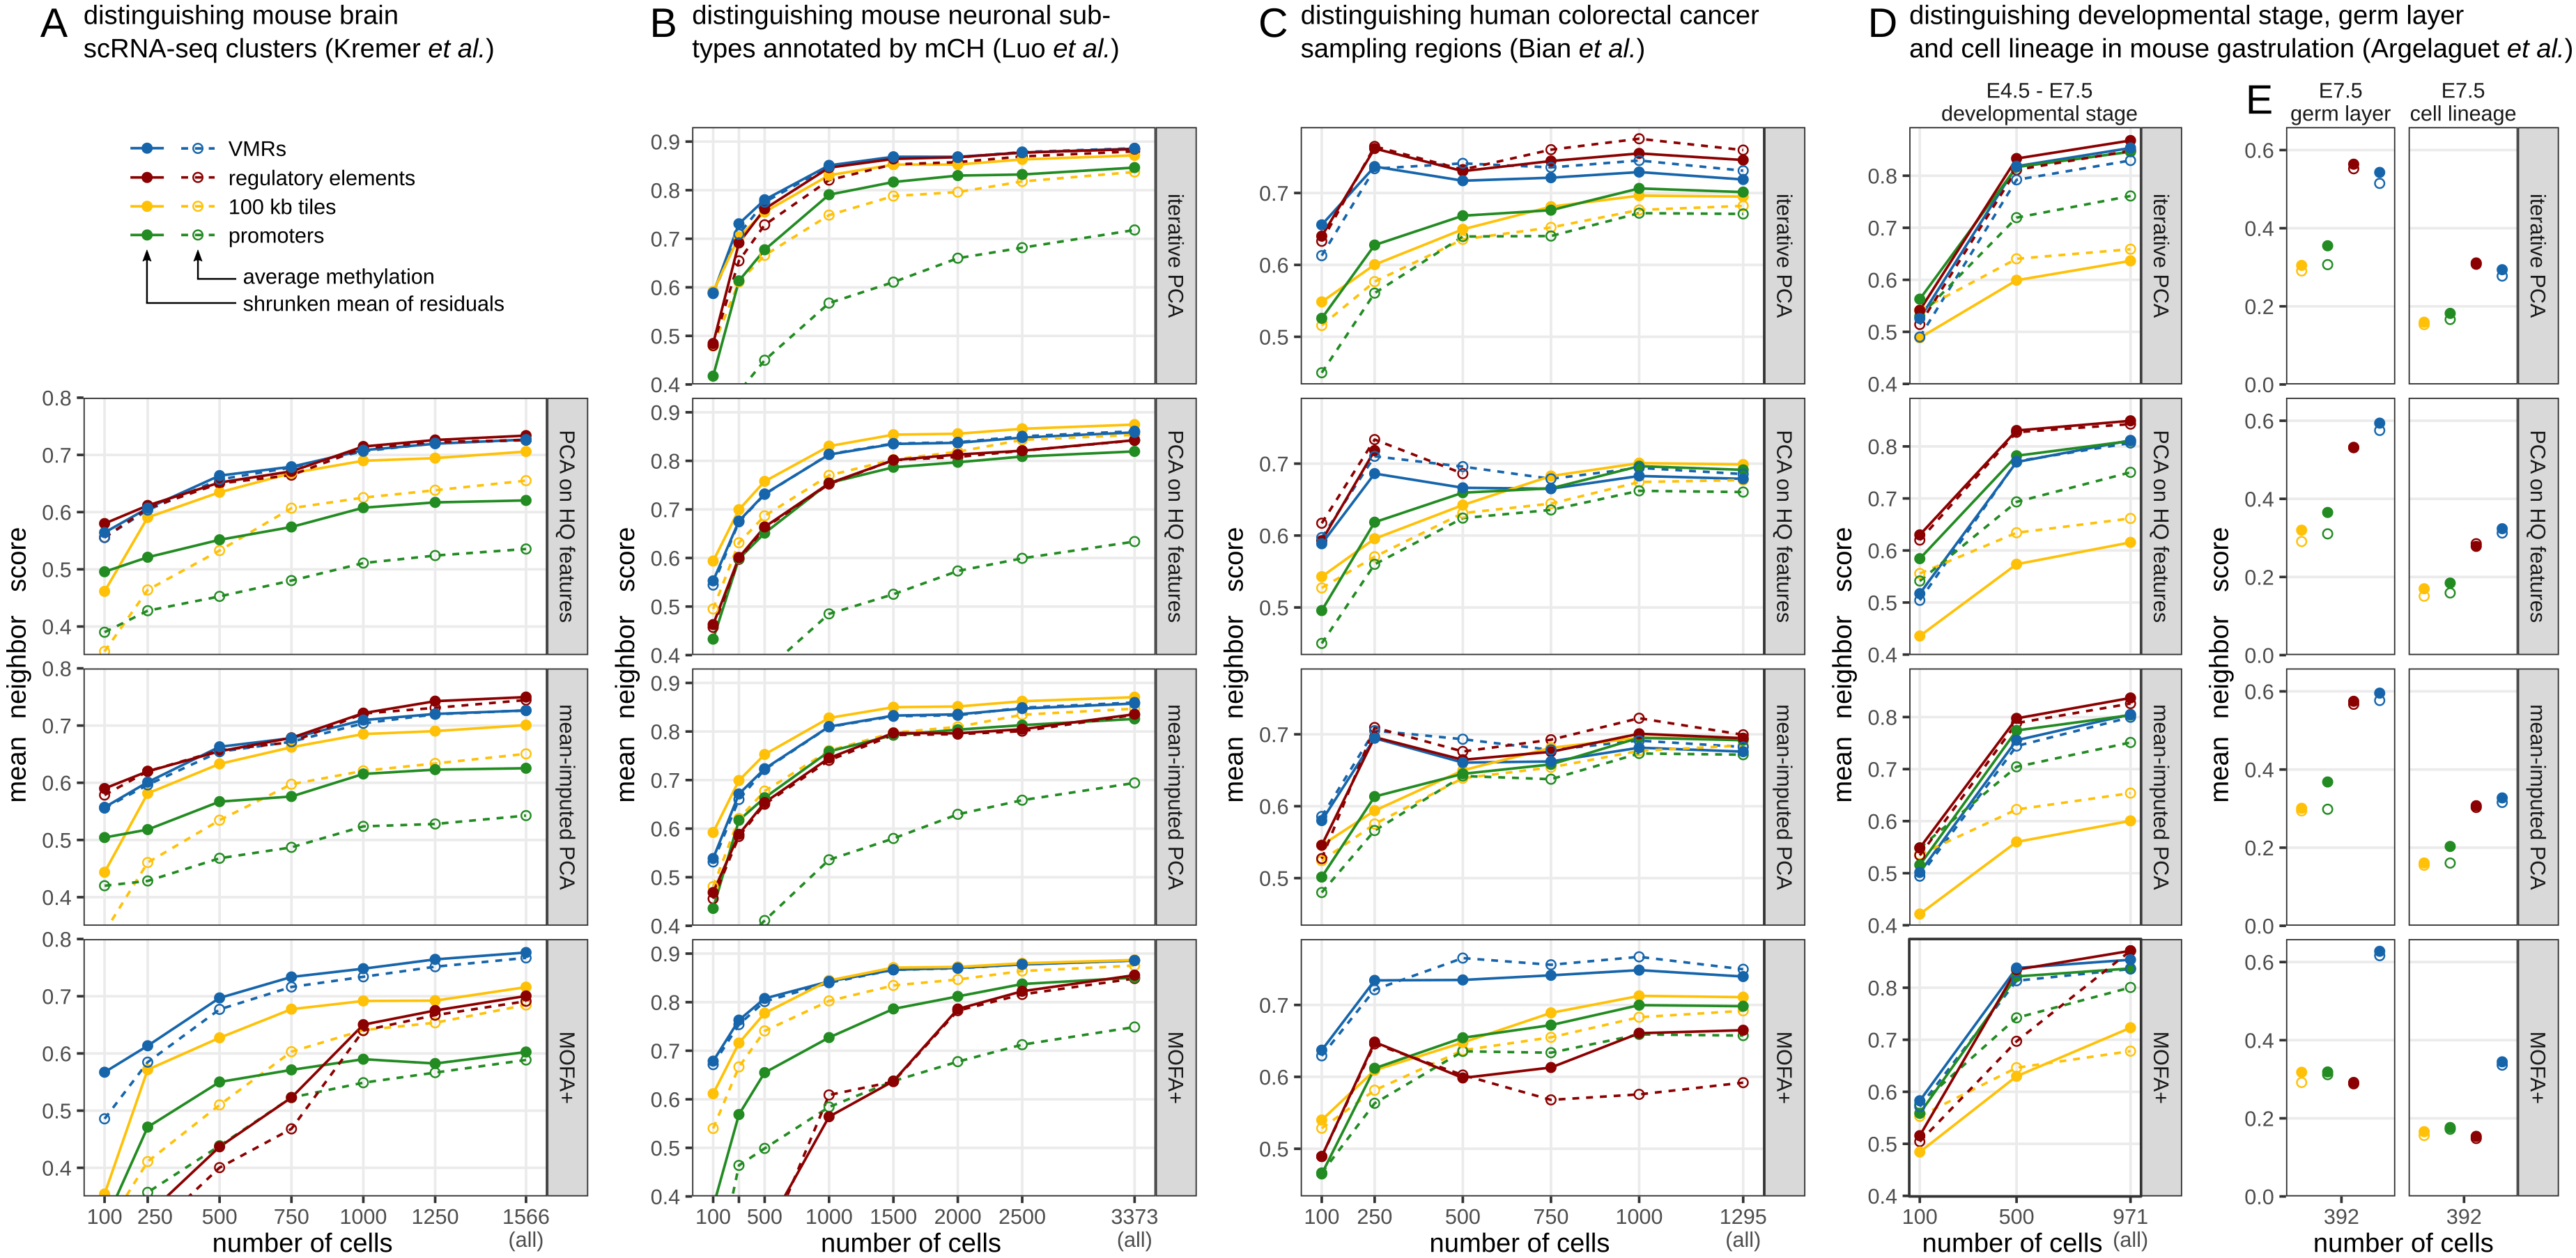
\includegraphics[width=0.4\textwidth]{figures/SFig_benchmark.png}
	\end{center}
	\captionof{figure}{\small \textbf{Benchmark of our methods on single-cell methylomes of neural subtypes of the murine frontal cortex}.\\
	Our methods were benchmarked on single-cell methylomes from \citet{luo2017single} as described in Fig.~\ref{fig:score}. 
	}
	\label{fig:score_luo}
\end{minipage}
\vspace{6ex}

\noindent%
\begin{minipage}{\linewidth}
    \begin{center}
        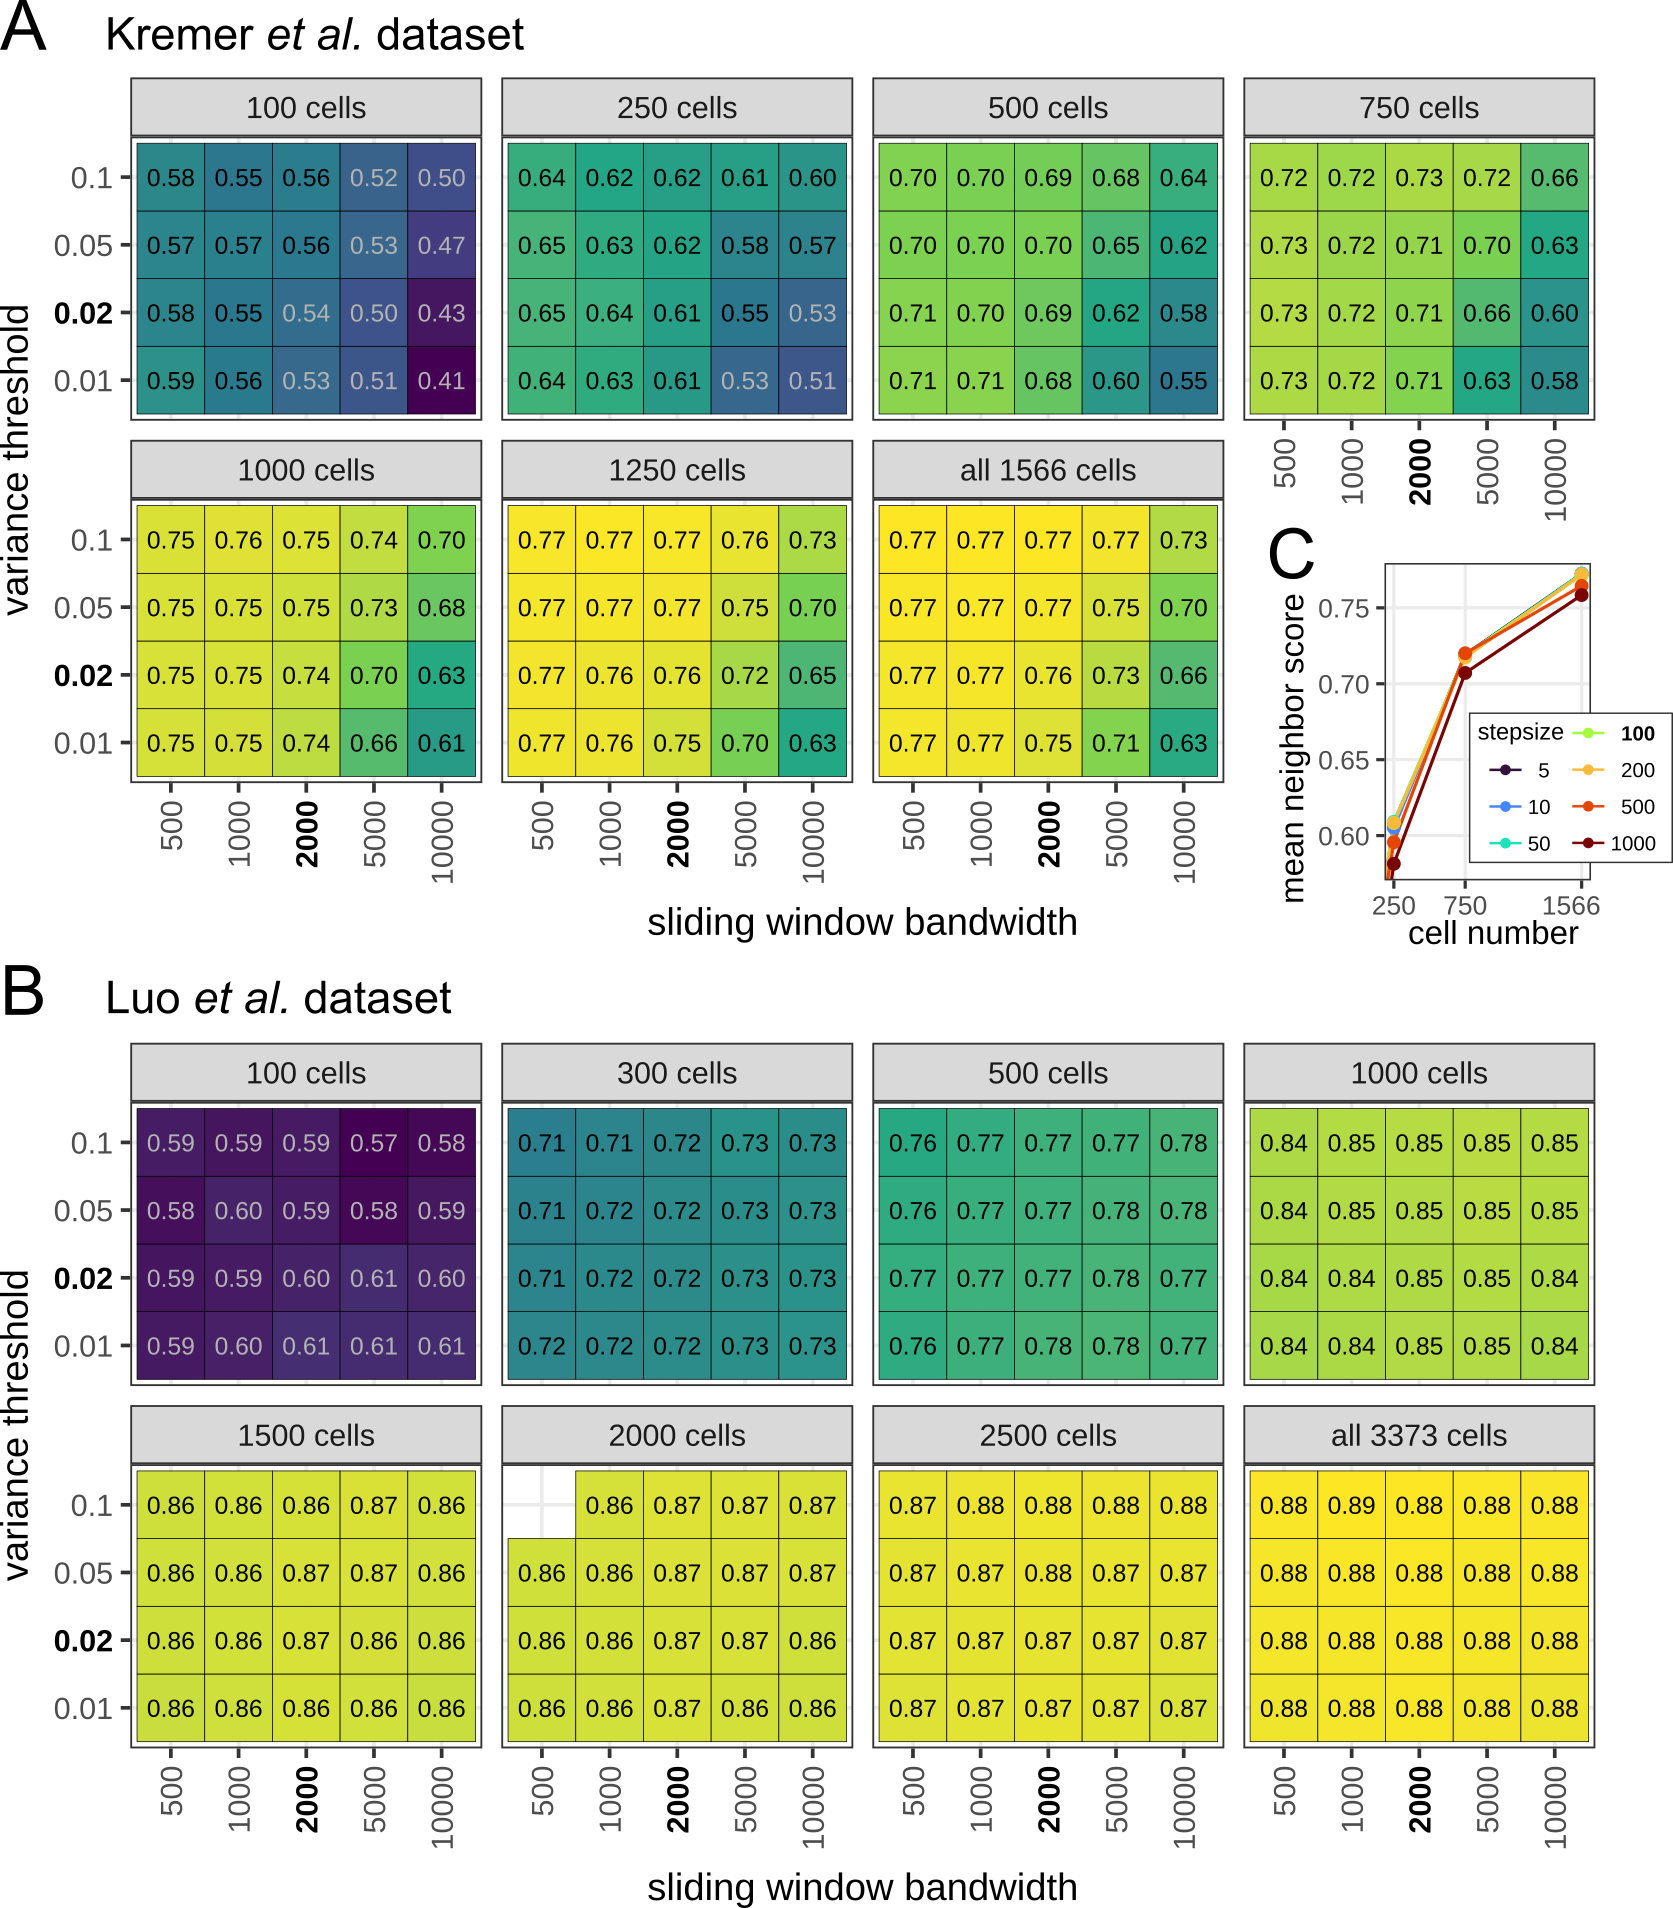
\includegraphics[width=.6\textwidth]{figures/SFig_parameter_sweep.png}
    \end{center}
    \captionof{figure}{\small \textbf{Effect of VMR detection parameters on separation of cell types}.\\
    \textbf{(A-B)} Mean neighbor scores obtained after analyzing single-cell methylomes from \citet{kremer_scnmt} (\textbf{A}) or \citet{luo2017single} (\textbf{B}) with our proposed methods.
    VMRs were detected with \texttt{scbs scan} using various sliding window bandwidths or variance thresholds, and on sub-samples of the full data sets.
    }
    \label{fig:sweep}
\end{minipage}

\end{document}